%!TEX program = pdflatex
%%%%%%%%%%%%%%%%%%%%%%%%%%%%%%%%%%%%%%%%%
% The Legrand Orange Book
% LaTeX Template
% Version 1.4 (12/4/14)
%
% This template has been downloaded from:
% http://www.LaTeXTemplates.com
%
% Original author:
% Mathias Legrand (legrand.mathias@gmail.com)
%
% License:
% CC BY-NC-SA 3.0 (http://creativecommons.org/licenses/by-nc-sa/3.0/)
%
% Compiling this template:
% This template uses biber for its bibliography and makeindex for its index.
% When you first open the template, compile it from the command line with the 
% commands below to make sure your LaTeX distribution is configured correctly:
%
% 1) pdflatex main
% 2) makeindex main.idx -s StyleInd.ist
% 3) biber main
% 4) pdflatex main x 2
%
% After this, when you wish to update the bibliography/index use the appropriate
% command above and make sure to compile with pdflatex several times 
% afterwards to propagate your changes to the document.
%
% This template also uses a number of packages which may need to be
% updated to the newest versions for the template to compile. It is strongly
% recommended you update your LaTeX distribution if you have any
% compilation errors.
%
% Important note:
% Chapter heading images should have a 2:1 width:height ratio,
% e.g. 920px width and 460px height.
%
%%%%%%%%%%%%%%%%%%%%%%%%%%%%%%%%%%%%%%%%%

%----------------------------------------------------------------------------------------
%	PACKAGES AND OTHER DOCUMENT CONFIGURATIONS
%----------------------------------------------------------------------------------------

\documentclass[11pt,fleqn]{book} % Default font size and left-justified equations

\usepackage[top=3cm,bottom=3cm,left=3.2cm,right=3.2cm,headsep=10pt,a4paper]{geometry} % Page margins

\usepackage[table,xcdraw]{xcolor} % Required for specifying colors by name
\definecolor{verde}{RGB}{51,153,51} % Define the color used for highlighting throughout the book
\definecolor{blue}{rgb}{0.2, 0.2, 0.6}
\definecolor{red}{rgb}{0.8, 0.0, 0.0}
\definecolor{green}{rgb}{0.0, 0.42, 0.24}

% Font Settings
\usepackage{avant} % Use the Avantgarde font for headings
%\usepackage{times} % Use the Times font for headings
\usepackage{mathptmx} % Use the Adobe Times Roman as the default text font together with math symbols from the Sym­bol, Chancery and Com­puter Modern fonts

\usepackage{microtype} % Slightly tweak font spacing for aesthetics
\usepackage[utf8]{inputenc} % Required for including letters with accents
\usepackage[T1]{fontenc} % Use 8-bit encoding that has 256 glyphs
\hyphenation{Mi-nis-té-ri-o}


% Index
\usepackage{calc} % For simpler calculation - used for spacing the index letter headings correctly
\usepackage{makeidx} % Required to make an index
\makeindex % Tells LaTeX to create the files required for indexing
\usepackage{verbatim}

\usepackage[colorinlistoftodos,prependcaption,textsize=tiny,linecolor=red,backgroundcolor=red!25,bordercolor=red]{todonotes}
\usepackage{epigraph}
\renewcommand{\textflush}{flushepinormal}
\setlength{\epigraphwidth}{0.8\textwidth}

\usepackage{nameref}
\usepackage{booktabs}
\usepackage{graphicx}
\usepackage{rotating}
\usepackage{float}
\usepackage{multirow}

\usepackage[normalem]{ulem}%tachado


% Bibliography
%\usepackage[backend=biber,style=authoryear,autocite=inline, citestyle=authoryear]{biblatex}
\usepackage[style=abnt]{biblatex}
\addbibresource{bibliography.bib} % BibTeX bibliography file
\defbibheading{bibempty}{}
\renewcommand*{\nameyeardelim}{\addcomma\space}

\newcommand{\VER}[1]{\begingroup\color{red}#1\endgroup}

\renewenvironment{quote}
{\small\list{}{\rightmargin=.1cm \leftmargin=2.5cm}%
	\item\relax}
{\endlist}


%----------------------------------------------------------------------------------------

%----------------------------------------------------------------------------------------
%	VARIOUS REQUIRED PACKAGES
%----------------------------------------------------------------------------------------
\usepackage{titlesec} % Allows customization of titles
\usepackage{graphicx} % Required for including pictures
\graphicspath{{Pictures/}} % Specifies the directory where pictures are stored
\usepackage{lipsum} % Inserts dummy text
\usepackage{tikz} % Required for drawing custom shapes
\usepackage[english,brazil]{babel} % English language/hyphenation
\usepackage{enumitem} % Customize lists
\setlist{nolistsep} % Reduce spacing between bullet points and numbered lists
\usepackage{booktabs} % Required for nicer horizontal rules in tables
\usepackage{eso-pic} % Required for specifying an image background in the title page

%----------------------------------------------------------------------------------------
%	MAIN TABLE OF CONTENTS
%----------------------------------------------------------------------------------------
\usepackage{titletoc} % Required for manipulating the table of contents
\contentsmargin{0cm} % Removes the default margin
% Chapter text styling
\titlecontents{chapter}[1.25cm] % Indentation
{\addvspace{20pt}\large\sffamily\bfseries} % Spacing and font options for chapters
{\color{verde!60}\contentslabel[\Large\thecontentslabel]{1.25cm}\color{verde}} % Chapter number
{}  
{\color{verde!60}\normalsize\sffamily\bfseries\;\titlerule*[.5pc]{.}\;\thecontentspage} % Page number
% Section text styling
\titlecontents{section}[1.25cm] % Indentation
{\addvspace{5pt}\sffamily\bfseries} % Spacing and font options for sections
{\contentslabel[\thecontentslabel]{1.25cm}} % Section number
{}
{\sffamily\hfill\color{black}\thecontentspage} % Page number
[]
% Subsection text styling
\titlecontents{subsection}[1.25cm] % Indentation
{\addvspace{15pt}\sffamily\small} % Spacing and font options for subsections
{\contentslabel[\thecontentslabel]{1.25cm}} % Subsection number
{}
{\sffamily\;\titlerule*[.5pc]{.}\;\thecontentspage} % Page number
[] 
%----------------------------------------------------------------------------------------
%	MINI TABLE OF CONTENTS IN CHAPTER HEADS
%----------------------------------------------------------------------------------------
% Section text styling
\titlecontents{lsection}[.05em] % Indendating
{\footnotesize\sffamily} % Font settings
{}
{}
{}
% Subsection text styling
\titlecontents{lsubsection}[.5em] % Indentation
{\normalfont\footnotesize\sffamily} % Font settings
{}
{}
{}
%----------------------------------------------------------------------------------------
%	PAGE HEADERS
%----------------------------------------------------------------------------------------
\usepackage{fancyhdr} % Required for header and footer configuration
\pagestyle{fancy}
\renewcommand{\chaptermark}[1]{\markboth{\sffamily\normalsize\bfseries\chaptername\ \thechapter.\ #1}{}} % Chapter text font settings
\renewcommand{\sectionmark}[1]{\markright{\sffamily\normalsize\thesection\hspace{2pt}#1}{}} % Section text font settings
\fancyhf{} \fancyhead[LE,RO]{\sffamily\normalsize\thepage} % Font setting for the page number in the header
%\fancyhead[LO]{\rightmark} % Print the nearest section name on the left side of odd pages
\fancyhead[RE]{\leftmark} % Print the current chapter name on the right side of even pages
\renewcommand{\headrulewidth}{0.5pt} % Width of the rule under the header
\addtolength{\headheight}{2.5pt} % Increase the spacing around the header slightly
\renewcommand{\footrulewidth}{0pt} % Removes the rule in the footer
\fancypagestyle{plain}{\fancyhead{}\renewcommand{\headrulewidth}{0pt}} % Style for when a plain pagestyle is specified
% Removes the header from odd empty pages at the end of chapters
\makeatletter
\renewcommand{\cleardoublepage}{
\clearpage\ifodd\c@page\else
\hbox{}
\vspace*{\fill}
\thispagestyle{empty}
\newpage
\fi}
%----------------------------------------------------------------------------------------
%	THEOREM STYLES
%----------------------------------------------------------------------------------------
\usepackage{amsmath,amsfonts,amssymb,amsthm} % For math equations, theorems, symbols, etc
\newcommand{\intoo}[2]{\mathopen{]}#1\,;#2\mathclose{[}}
\newcommand{\ud}{\mathop{\mathrm{{}d}}\mathopen{}}
\newcommand{\intff}[2]{\mathopen{[}#1\,;#2\mathclose{]}}
\newtheorem{notation}{Notation}[chapter]
%----------------------------------------------------------------------------------------
%	DEFINITION OF COLORED BOXES
%----------------------------------------------------------------------------------------
\RequirePackage[framemethod=default]{mdframed} % Required for creating the theorem, definition, exercise and corollary boxes
%----------------------------------------------------------------------------------------
%	REMARK ENVIRONMENT
%----------------------------------------------------------------------------------------
\newenvironment{remark}{\par\vspace{10pt}\small % Vertical white space above the remark and smaller font size
\begin{list}{}{
\leftmargin=35pt % Indentation on the left
\rightmargin=25pt}\item\ignorespaces % Indentation on the right
\makebox[-2.5pt]{\begin{tikzpicture}[overlay]
\node[draw=verde!60,line width=1pt,circle,fill=verde!25,font=\sffamily\bfseries,inner sep=2pt,outer sep=0pt] at (-15pt,0pt){\textcolor{verde}{R}};\end{tikzpicture}} % Orange R in a circle
\advance\baselineskip -1pt}{\end{list}\vskip5pt} % Tighter line spacing and white space after remark
%----------------------------------------------------------------------------------------
%	SECTION NUMBERING IN THE MARGIN
%----------------------------------------------------------------------------------------
\makeatletter
\renewcommand{\@seccntformat}[1]{\llap{\textcolor{verde}{\csname the#1\endcsname}\hspace{1em}}}                    
\renewcommand{\section}{\@startsection{section}{1}{\z@}
{-4ex \@plus -1ex \@minus -.4ex}
{1ex \@plus.2ex }
{\normalfont\large\sffamily\bfseries}}
\renewcommand{\subsection}{\@startsection {subsection}{2}{\z@}
{-3ex \@plus -0.1ex \@minus -.4ex}
{0.5ex \@plus.2ex }
{\normalfont\sffamily\bfseries}}
\renewcommand{\subsubsection}{\@startsection {subsubsection}{3}{\z@}
{-2ex \@plus -0.1ex \@minus -.2ex}
{.2ex \@plus.2ex }
{\normalfont\small\sffamily\bfseries}}                        
\renewcommand\paragraph{\@startsection{paragraph}{4}{\z@}
{-2ex \@plus-.2ex \@minus .2ex}
{.1ex}
{\normalfont\small\sffamily\bfseries}}
%----------------------------------------------------------------------------------------
%	HYPERLINKS IN THE DOCUMENTS
%----------------------------------------------------------------------------------------
% For an unclear reason, the package should be loaded now and not later
\usepackage{hyperref}
\hypersetup{hidelinks,backref=true,pagebackref=true,hyperindex=true,colorlinks=false,breaklinks=true,
	urlcolor=verde,bookmarks=true,bookmarksopen=false,pdftitle={Title},pdfauthor={Author}}
%----------------------------------------------------------------------------------------
%	CHAPTER HEADINGS
%----------------------------------------------------------------------------------------
% The set-up below should be (sadly) manually adapted to the overall margin page septup controlled by the geometry package loaded in the main.tex document. It is possible to implement below the dimensions used in the goemetry package (top,bottom,left,right)... TO BE DONE
\newcommand{\thechapterimage}{}
\newcommand{\chapterimage}[1]{\renewcommand{\thechapterimage}{#1}}
% Numbered chapters with mini tableofcontents
\def\thechapter{\arabic{chapter}}
\def\@makechapterhead#1{
\thispagestyle{empty}
{\centering \normalfont\sffamily
\ifnum \c@secnumdepth >\m@ne
\if@mainmatter
\startcontents
\begin{tikzpicture}[remember picture,overlay]
\node at (current page.north west)
{\begin{tikzpicture}[remember picture,overlay]
\node[rounded corners=5pt,anchor=north west,inner sep=0pt] at (0,0) {\includegraphics[width=\paperwidth]{\thechapterimage}};
%%%%%%%%%%%%%%%%%%%%%%%%%%%%%%%%%%%%%%%%%%%%%%%%%%%%%%%%%%%%%%%%%%%%%%%%%%%%%%%%%%%%%
%Tamanho do mini table of contents
\fill[color=verde!10!white,opacity=.6] (.5cm,0) rectangle (9.9cm,-13cm);
%Conteúdo do mini table of contents 
\node[rounded corners=10pt,anchor=north west] at (1.1cm,.35cm) {\parbox[t][10cm][t]{10cm}{\huge\bfseries\flushleft \printcontents{l}{1}{\setcounter{tocdepth}{2}}}};
%Titulo do capitulo
\draw[anchor=west] (10cm,-10cm) node [rounded corners=5pt,fill=verde!10!white,text opacity=1,draw=verde,draw opacity=1,line width=1.5pt,fill opacity=.6,inner sep=12pt]{\huge\sffamily\bfseries\textcolor{black}{\thechapter. #1\strut\makebox[20cm]{}}};
%%%%%%%%%%%%%%%%%%%%%%%%%%%%%%%%%%%%%%%%%%%%%%%%%%%%%%%%%%%%%%%%%%%%%%%%%%%%%%%%%%%%%
\end{tikzpicture}};
\end{tikzpicture}}
\par\vspace*{230\p@}
\fi
\fi}
% Unnumbered chapters without mini tableofcontents (could be added though) 
\def\@makeschapterhead#1{
\thispagestyle{empty}
{\centering \normalfont\sffamily
\ifnum \c@secnumdepth >\m@ne
\if@mainmatter
\begin{tikzpicture}[remember picture,overlay]
\node at (current page.north west)
{\begin{tikzpicture}[remember picture,overlay]
\node[anchor=north west,inner sep=0pt] at (0,0) {\includegraphics[width=\paperwidth]{\thechapterimage}};
\draw[anchor=west] (2cm,-9cm) node [rounded corners=5pt,fill=verde!10!white,fill opacity=.6,inner sep=12pt,text opacity=1,draw=verde,draw opacity=1,line width=1.5pt]{\huge\sffamily\bfseries\textcolor{black}{#1\strut\makebox[22cm]{}}};
\end{tikzpicture}};
\end{tikzpicture}}
\par\vspace*{230\p@}
\fi
\fi
}
\makeatother % Insert the commands.tex file which contains the majority of the structure behind the template

\begin{document}

\let\cleardoublepage\clearpage

\renewcommand{\chaptername}{Capítulo}
\renewcommand{\figurename}{Fig.}

%----------------------------------------------------------------------------------------
%	TITLE PAGE
%----------------------------------------------------------------------------------------
\begingroup
	\thispagestyle{empty}
	
	\AddToShipoutPicture*{\put(0,0){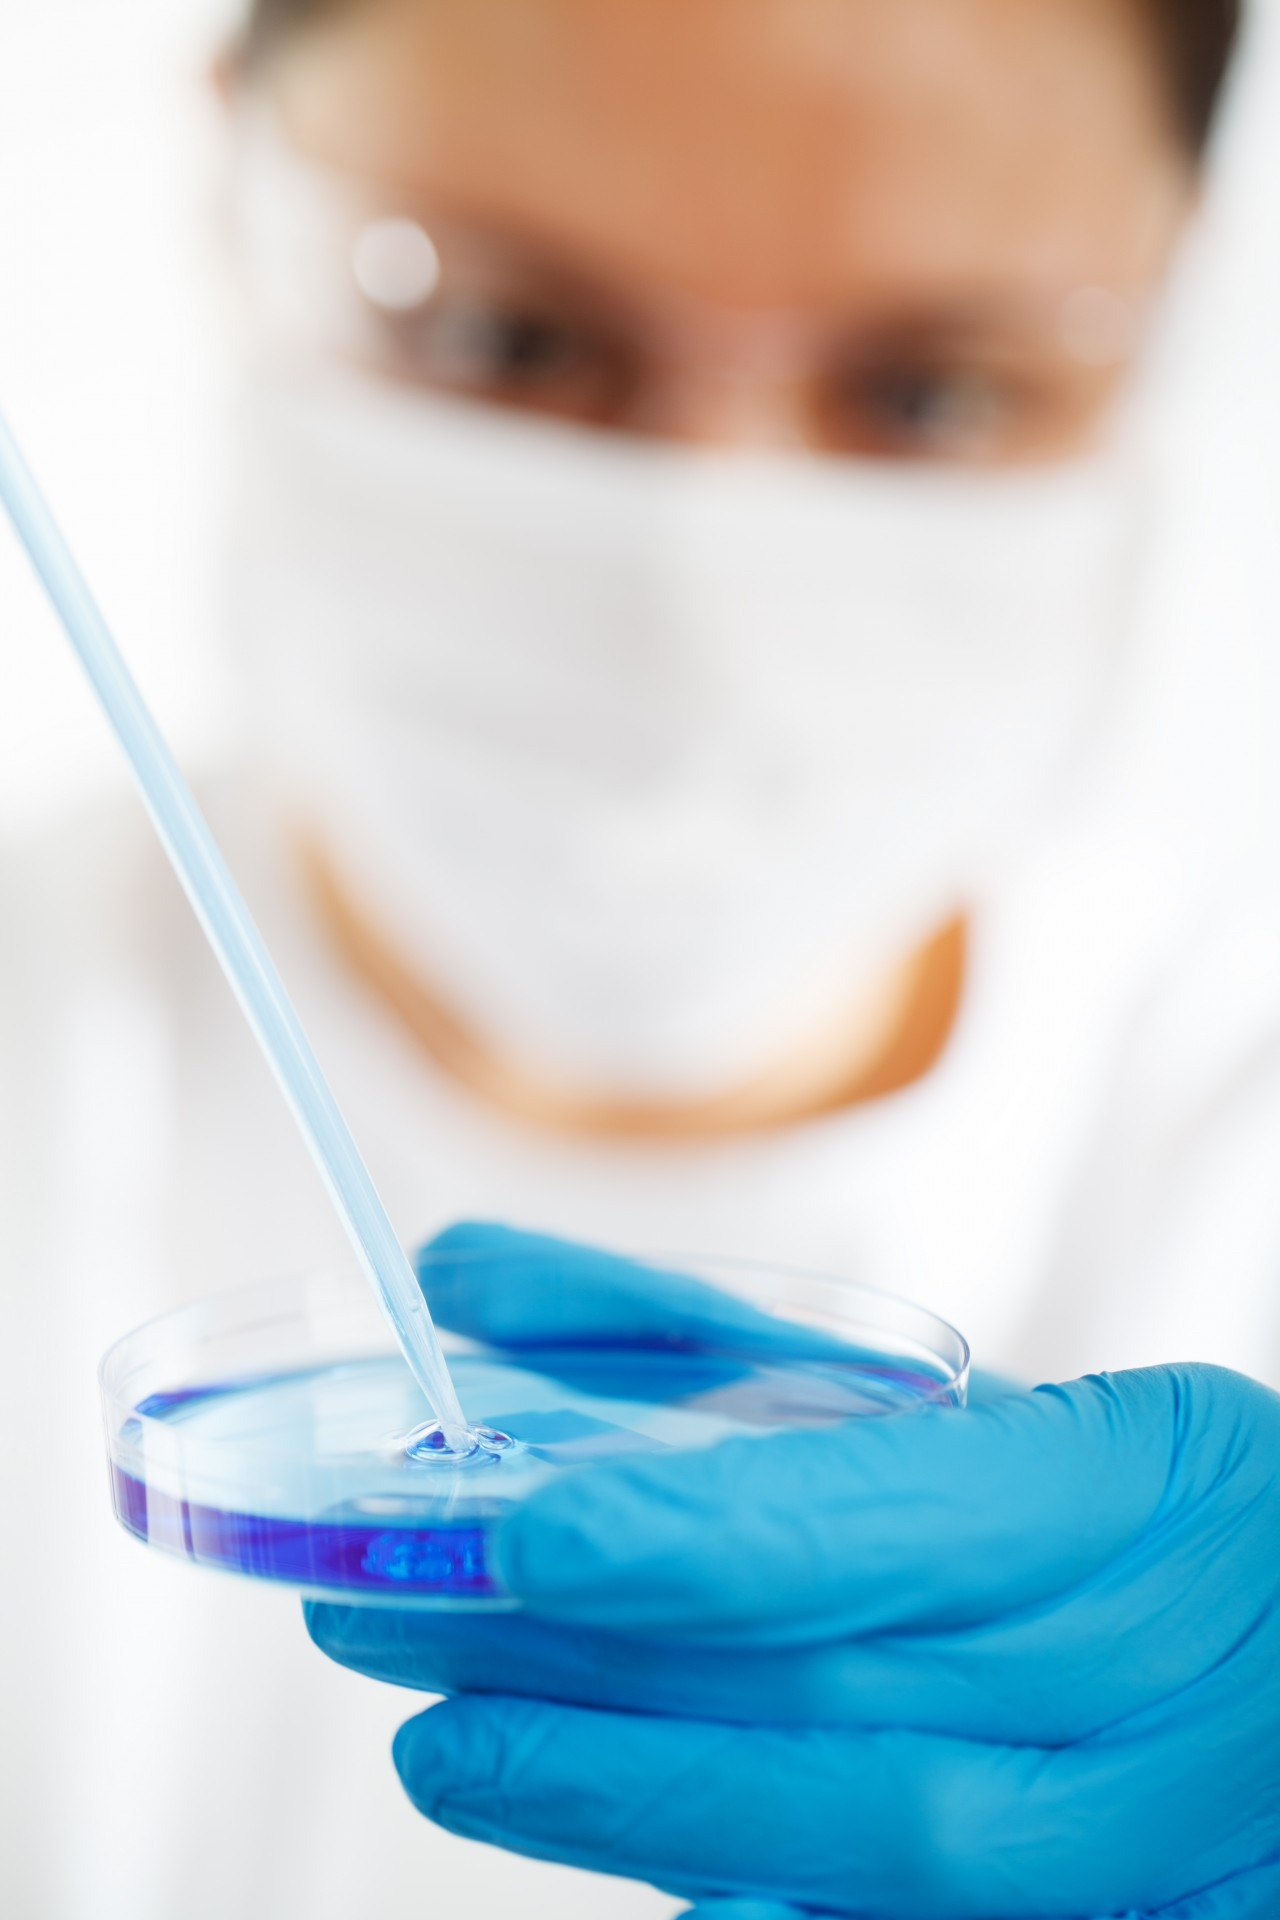
\includegraphics[scale=1]{capa}}} % Image background
	
	\AddToShipoutPicture*{\put(116,650){
\includegraphics[scale=.75]{brasao.png}}} % Image background
	
	\AddToShipoutPicture*{\put(244,200){
\includegraphics[scale=0.2]{ifgvertical}}} % Image background
	
	\vspace*{4.5cm}
	
	\centering
	\par
	{\Huge Projeto Pedagógico}\vspace*{1.5cm}
	\par
	\fontsize{40}{40}
	\selectfont
	Técnico Integrado em Tempo Integral em Biotecnologia\vspace*{10cm}
	\par
	{\Huge 2019}
	\par
\endgroup
\pagebreak

%----------------------------------------------------------------------------------------
%	PEOPLE PAGE
%----------------------------------------------------------------------------------------
\chapterimage{banner3} % Chapter heading image
\begin{center}
	\par
	{\large PRESIDENTE DA REPÚBLICA \\ Jair Messias Bolsonaro}\vspace*{1cm}
	\par
	{\large MINISTRO DA EDUCAÇÃO \\ \VER{Nome do Ministro} }\vspace*{1cm}
	\par
	{\large SECRETÁRIO DE EDUCAÇÃO PROFISSIONAL E TECNOLÓGICA \\ Alexandro Ferreira de Souza}\vspace*{1cm}
	\par
	{\large REITOR DO INSTITUTO FEDERAL DE GOIÁS \\ Jerônimo Rodrigues da Silva}\vspace*{1cm}
	\par
	{\large PRÓ-REITOR DE PESQUISA E PÓS-GRADUAÇÃO \\ \VER{Nome da(o) pró-reitor(a)} }\vspace*{1cm}
	\par
	{\large DIRETORIA DE PÓS-GRADUAÇÃO \\ \VER{Nome da(o) pró-reitor(a)} }\vspace*{1cm}
	\par
	{\large COORDENADOR DO CURSO \\ Waldeyr Mendes Cordeiro da Silva}\vspace*{1cm}
\end{center}

\chapterimage{banner3} % Chapter heading image
\renewcommand\contentsname{Sumário}
\tableofcontents

%----------------------------------------------------------------------------------------
%	CHAPTER
%----------------------------------------------------------------------------------------
\chapterimage{01.jpg} % Chapter heading image
\chapter{Apresentação}
\vspace{6em}
\begin{flushright}
	\textit{ }
\end{flushright}
\vspace{12em}
\indent


\section{Identificação do Curso}
\begin{itemize}
	\item \textbf{Instituição Proponente:} Instituto Federal de Educação, Ciência e Tecnologia de Goiás
	\item \textbf{Nome do curso:} Técnico Integrado em Tempo Integral em Biotecnologia
	\item \textbf{Carga Horária do Curso:}~\VER{3304} horas
	\item \textbf{Forma de oferta:} Presencial
	\item \textbf{Duração:} 3 anos
	\item \textbf{Número de Vagas:} 30 vagas anuais
	\item \textbf{Local de Oferta:} Instituto Federal de Goiás - Câmpus Formosa
	\item \textbf{Reitor:} Jerônimo Rodrigues da Silva
	\item \textbf{Pró-Reitora de Ensino:} Oneida Cristina Gomes Barcelos Irigon
	\item \textbf{Pró-Reitor de Pesquisa, Pós-Graduação e Inovação:} \VER{Nome da(o) pró-reitor(a)}
	\item \textbf{Diretoria de Pós-Graduação:} \VER{Nome da(o) diretor(a)}
\end{itemize}

%-----------------------------------------------
\newpage  
%------------------------------------------------
\section{Comissão Organizadora}
	\begin{itemize}[label=\bfseries]
		\item \nameref{AdrianoDarosci}
		\item ...
		\item \nameref{WaldeyrMendes}
	\end{itemize}

%----------------------------------------------------------------------------------------
%	CHAPTER
%----------------------------------------------------------------------------------------
\chapterimage{02.jpg} % Chapter heading image

\chapter{Introdução}
\vspace{6em}
\begin{flushright}
	\textit{\textcolor{white}{Foto: Adriano Darosci}}
\end{flushright}
\vspace{12em}
\indent

De acordo com a Convenção sobre Diversidade Biológica da ONU em 1992, biotecnologia é qualquer aplicação tecnológica que use sistemas biológicos, organismos vivos ou derivados destes, para fazer ou modificar produtos ou processos para usos específicos.
A biotecnologia abrange processos microbiológicos, organismos vivos e biossistemas para produzir novas práticas e produtos.
Em todo o mundo, incluindo o Brasil, a biotecnologia vêm permeando, modificando e impulsionando inúmeras áreas da economia~\cite{dias2017bioeconomiabrasil}, incluindo a bioeconomia, que pode ser entendida como a economia baseada em materiais, químicos e energia derivada de fontes biológicas renováveis~\cite{mccormick2013bioeconomy}.
O desenvolvimento da bioeconomia depende de desenvolver capacidades para explorar a biodiversidade. 
Entretanto, a sustentabilidade não é uma característica inerente da bioeconomia~\cite{pfau2014visions}, o que traz a necessidade de pesquisa em abordagens que busquem explorar o potencial biotecnológico de forma integrada com sua preservação.

O Projeto Pedagógico do Curso – PPC está organizado a partir dos Eixos Tecnológicos constantes do Catálogo Nacional dos Cursos Técnicos - CNTC~\cite{CatalogoCursosTecnicos2016}.
Apesar de ligado ao Eixo de Produção Industrial, é um curso altamente interdisciplinar com possibilidades de verticalização para cursos de graduação no itinerário formativo superior de tecnologia em biotecnologia, superior de tecnologia em saneamento ambiental, bacharelado ou licenciatura em ciências biológicas, bacharelados em biomedicina, farmácia, nutrição, em engenharia de alimento, em engenharia química, em biotecnologia e em engenharia ambiental.

\section{Justificativa}
\indent

Desenvolver a educação profissional e tecnológica como processo educativo e investigativo de geração e adaptação de soluções técnicas e tecnológicas às demandas sociais e peculiaridades regionais está entre as finalidades e características dos Institutos Federais~\cite{Lei11892De2008}. 
A Lei 11.892 de 2008~\cite{Lei11892De2008} indica ainda como objetivo que os Institutos Federais devem ministrar educação profissional técnica de nível médio, prioritariamente na forma de cursos integrados ao Ensino Médio.

Dessa forma, alinhado às demandas regionais e nacionais, o IFG câmpus Formosa, vem ofertando o curso de Biotecnologia desde 2011 com uma eficiência acadêmica superior a 86\%.
O curso já passou por uma atualização em 2014 e este projeto pedagógico traz sua segunda atualização, com vistas a adequar-se simultaneamente às recentes mudanças promovidas pela reforma do Ensino Médio, ao mesmo tempo que busca manutenir e melhorar seus números de eficiência acadêmica tal como definido em Lei~\cite{Lei13005De2014} e no Plano de Desenvolvimento Institucional 2019-2023 do IFG~\cite{Resolucao32De2018}.

Além dos aspectos legais, esta atualização promove um novo olhar pedagógico na organização didática das disciplinas.
Essas mudanças são pautadas pelo perfil do egresso do curso, o qual foi construído de forma colaborativa pela Comunidade Acadêmica.
Nesse sentido, a matriz curricular foi reconcebida para proporcionar meios de alcançar tal perfil de egresso.
O perfil do egresso leva em conta uma formação integral que promova o desenvolvimento do estudante na sua totalidade, considerando as dimensões físico-psíquico-cognitiva, histórica, social e profissional.

Em relação a aspectos sócioeconômicos, a cidade de Formosa conta com uma população urbana de 106.462 habitantes de acordo com a PMAD – Pesquisa Metropolitana por Amostra de Domicílios~\cite{pmad2017codeplan}, onde cerca de 40\% são jovens até 24 anos, 20\% dos quais entre 15 e 24 anos. 
Essa faixa da população é o público alvo deste curso Técnico Integrado ao Ensino Médio juntamente com os demais cursos superiores do IFG.

\subsection{Objetivos}
Em consonância com as Bases Curriculares Nacionais, Diretrizes para o Ensino Médio Profissionalizante, e a demanda por profissionais capacitados em Biotecnologia, os objetivos do curso são:
\begin{itemize}
\item Atender às expectativas dos estudantes e às demandas da sociedade contemporânea para a formação no Ensino Médio e Profissional
\item Garantir aos estudantes o protagonismo no processo de escolarização, reconhecendo-os como interlocutores legítimos sobre currículo, ensino e aprendizagem
\item Proporcionar experiências e processos que lhes garantam as aprendizagens necessárias para a leitura da realidade, o enfrentamento dos novos desafios da contemporaneidade (sociais, econômicos e ambientais) e a tomada de decisões éticas e fundamentadas
\item Desenvolver competências e habilidades relacionadas à área de Biotecnologia para atuação profissional
\end{itemize}

%\section{Requisitos para Acesso ao Curso}
%
%\todo[inline]{Texto...}


\section{Perfil do Egresso}\label{Perfil}
\indent

O \textbf{Técnico em Biotecnologia} egresso do \textbf{Curso Técnico Integrado em Tempo Integral em Biotecnologia} possui, mas não limita-se, às seguintes habilidades:

\begin{enumerate}
	\item\label{perfil01} Executa, controla e monitora processos e atividades laboratoriais de biotecnologia e biociências em diversos setores indústria, meio-ambiente, agropecuária, saúde humana e animal.
	\item\label{perfil02} Controla a qualidade e a compra de matérias-primas, insumos e produtos.
	\item\label{perfil03} Prepara materiais, meios de cultura, soluções e reagentes.
	\item\label{perfil04} Prepara amostras e cultiva \textit{in vivo} e \textit{in vitro} microrganismos, células e tecidos animais e vegetais.
	\item\label{perfil05} Opera a criação e manejo de animais de experimentação.
	\item\label{perfil06} Analisa substâncias e materiais biológicos.
	\item\label{perfil07} Extrai, replica e quantifica biomoléculas.
	\item\label{perfil08} Realiza a produção de imunobiológicos, vacinas, diluentes, kits de diagnóstico e bioprocessos industriais.
	\item\label{perfil09} Colabora nas atividades de perícia criminal e investigação genética. 
	\item\label{perfil10} Desenvolve pesquisa em biotecnologia.
	\item\label{perfil11} Compreende e domina os fundamentos científico-tecnológicos do seu trabalho.
	\item\label{perfil12} Respeita as diversidades e os direitos humanos e tem atitude ética no trabalho e fora dele.
	\item\label{perfil13} Compreende e tem senso críticos frente aos projetos políticos de desenvolvimento nacional.
	\item\label{perfil14} Tem compromisso com a democracia e a responsabilidade social e ambiental.
	\item\label{perfil15} Cumpre da legislação ambiental.
	\item\label{perfil16} Avalia tendências no desenvolvimento da ciência e da tecnologia.
	\item\label{perfil17} Compreende a importância e impacto do seu trabalho.
	\item\label{perfil18} Usa a linguagem para a cidadania e profissão.
	\item\label{perfil19} Trabalha em equipe e conhece planejamento estratégico, iniciativa e liderança.
	\item\label{perfil20} Atualiza-se mantendo-se criativo e responsável.
\end{enumerate}


\subsection{Campo de atuação}
\indent

O campo de atuação inclui, mas não limita-se a empresas, indústrias, agroindústrias, instituições de pesquisa, ensino e desenvolvimento em biociências e produtos biotecnológicos.
Laboratórios de controle de qualidade de biomoléculas, de bioprocessos, de biologia molecular, de toxicologia, e de biodiagnósticos.%análises clínicas. 
Bancos de materiais biológicos e de genes. 
Empresas de consultorias, assistência técnica, comercialização de insumos e equipamentos utilizados na área de biociências e biotecnologia. 
Indústrias alimentícias, de cosméticos, bebidas e farmacêutica. 
Laboratório de agropecuária e ambiental. 
Estações de monitoramento e tratamento da água. 
Escritórios de patentes biotecnológicas. 
Empreendimento próprio.

\subsection{Ocupações CBO associadas}
\indent

325305-Técnico em biotecnologia. 

325310-Técnico em imunobiológicos.

\subsection{Normas associadas ao exercício profissional}
\indent

Lei nº 11.105/2005. 

Decreto nº 5.591/2005. 

Decreto nº 5.705/2006. 

Decreto nº 5.950/2006. 

Decreto nº 6.041/2007.

Decreto nº 6.925/2009. 

\subsection{Possibilidades de verticalização para cursos de graduação no itinerário formativo}

Curso superior de Tecnologia em Biotecnologia. 
Curso superior de Tecnologia em Saneamento Ambiental. 
Bacharelado em Ciências Biológicas. 
Bacharelado em Biomedicina. 
Bacharelado em Farmácia. 
Bacharelado em Nutrição. 
Bacharelado em Engenharia de Alimentos. 
Bacharelado em Engenharia Química. 
Bacharelado em Biotecnologia. 
Bacharelado em Engenharia Ambiental.

%----------------------------------------------------------------------------------------
%	CHAPTER
%----------------------------------------------------------------------------------------
\chapterimage{03.jpg} % Chapter heading image

\chapter{Organização do Curso}
\vspace{6em}
\begin{flushright}
	\textit{\textcolor{white}{``O homem, por ser inacabado, tende à perfeição. A educação é, portanto, um
			processo contínuo que só acaba com a morte'' (FURTER, 1973).}}
\end{flushright}
\vspace{12em}

\section{Forma de Oferta}\label{carga}
\indent

As Diretrizes Curriculares Nacionais para o Ensino Médio~\cite{Resolucao032018}, recentemente atualizadas, em consonância com a Lei de Diretrizes e Bases da Educação~\cite{Lei19394De1996}, trazem em seu Capítulo II as formas de Oferta e Organização Curricular. 
De acordo com as Diretrizes Curriculares Nacionais para o Ensino Médio, entre outros:

\begin{itemize}
	\item A oferta do Ensino Médio deve ser assegurada para todos os estudantes, sejam adolescentes,
	jovens ou adultos;
	\item O Ensino Médio pode organizar-se em tempos escolares de vários formatos:
	\begin{itemize}
		\item Séries anuais;
		\item Períodos Semestrais;
		\item Ciclos;
		\item Módulos;
		\item Sistema de Créditos;
		\item Alternância Regular de Períodos de estudos;
		\item Grupos não seriados com base na idade, competências e outros critérios;
	\end{itemize}
	\item O Ensino Médio deverá ter três anos no mínimo.
	\item A Educação a Distância pode ser usada para compor a carga horária do Ensino Médio Diurno na proporção de até 20\%;
\end{itemize}

Desta forma, o Curso Técnico Integrado ao Ensino Médio em Biotecnologia, em consonância com as mais recentes reestruturações do ensino, funcionará em período matutino e vespertino.

\subsection{Quantidade de Vagas}
\indent

30 (trinta) vagas anuais. 


\subsection{Forma de ingresso}

O ingresso nos cursos da educação profissional técnica de nível médio integrada ao ensino médio dar-se-á anualmente, por processo seletivo, somente para aqueles que tenham concluído o ensino fundamental, conforme previsto em edital de seleção~\cite{Resolucao22De2011}.

O ingresso por transferência para alunos regularmente matriculados em cursos da educação profissional técnica de nível médio integrada ao ensino médio dos campi do IFG ou oriundos de cursos da educação profissional técnica de nível médio integrada ao ensino médio de outras instituições públicas de ensino, dar-se-á somente a partir do segundo período dos cursos, mediante a existência de vagas, sujeitos à complementação de estudos, devendo ser requerido nas datas estabelecidas no calendário acadêmico da Instituição.
Não serão recebidas transferências de alunos em regime de dependência ou sujeito a estudos de recuperação~\cite{Resolucao22De2011}.

O aluno admitido por transferência deverá cursar as adaptações curriculares no curso por acompanhamento do Departamento responsável pelas disciplinas, por meio das coordenações de cursos e áreas no ano de ingresso no curso~\cite{Resolucao22De2011}.

A admissão por reingresso no curso será permitida uma única vez, mediante a existência de vaga, prazo legal para a conclusão do curso, condicionada as adaptações curriculares decorrentes de alteração na matriz curricular do curso, devendo ser requerida nas datas estabelecidas no calendário acadêmico da Instituição.
A solicitação de reingresso fora do curso de origem somente será admitida quando da extinção do mesmo.
Em cursos que exijam teste de habilidade específica como requisito de acesso somente poderá ser concedida mediante a aprovação em teste específico.
Nas solicitações de reingresso serão atendidos prioritariamente os alunos que obtiveram maior aproveitamento acadêmico nos cursos de origem~\cite{Resolucao22De2011}..


\subsection{Matrícula}

A matrícula de ingresso no curso será efetivada mediante a apresentação de toda a documentação exigida no edital público~\cite{Resolucao22De2011}..

\subsection{Duração e Carga Horária}
\indent

O Curso tem duração total de~\VER{3304} horas distribuídas em três anos.
A carga horária total está assim distruída:
\begin{itemize}
	\item \VER{3024} horas de Disciplinas
	\item \VER{160} horas de Estágio Curricular
	\item \VER{120} horas de Atividades Complementares
\end{itemize}

A duração mínima é de 3 (três) anos e o prazo máximo de integralização dos cursos da educação profissional técnica de nível médio integrado ao ensino médio é do dobro do tempo da sua duração. 
Logo, o máximo será de 6 (seis) anos, em conformidade com a legislação vigente. 
Após o prazo previsto por lei o aluno terá que se submeter a novo processo seletivo, caso deseje concluí-lo.


\section{Matriz Curricular}\label{matriz}
\indent
%
%Esta é uma disciplina de ementa aberta que visa assegurar tempos e espaços para que os estudantes reflitam sobre suas experiências e aprendizagens individuais e interpessoais, de modo a valorizarem o conhecimento, confiarem em sua capacidade de aprender, e identificarem e utilizarem estratégias mais eficientes a seu aprendizado~\cite{BNCC2019}.
%

A distribuição das disciplinas na matriz curricular foi fruto de construção coletiva e considera Ensino, Pesquisa e Extensão de forma indissociável, tal qual preconiza  a Resolução CNE/CEB nº 6, de Setembro de 2012~\cite{Resolucao06De2012}.
As disciplinas estão organizadas em séries anuais (Tabela~\ref{tab:matriz}), conforme sua densidade tecnológica.
Densidade tecnológica é um termo utilizado para qualificar um eixo tecnológico, ou um curso de educação profissional referindo-se a um construto teórico-metodológico. 
A densidade tecnológica aqui, refere-se à distribuição e à concentração de componentes tecnológicos por grades curriculares relativamente à carga horária, à intensidade da verticalização científica exigida pela complexidade tecnológica dos conteúdos trabalhados, à amplitude da cadeia tecnológica envolvida na proposta curricular de um curso, à combinação e articulação entre tecnologias tradicionais e modernas~\cite{Machado2010}.

\begin{table}[H]
	\centering
	\caption{Matriz Curricular do Curso Técnico em Biotecnologia Integrado ao Ensino Médio em Tempo Integral.}
	\label{tab:matriz}
	\resizebox{\textwidth}{!}{%
		\begin{tabular}{|l|l|l|l|l|l|}
			\hline
			Núcleo                     & Disciplinas                                       & 1º Ano     & 2º Ano    & 3º Ano    & CH Totais \\ \hline
			
			\multirow{12}{*}{Básico}
			& \nameref{disc:artes}                                                         & 2          & 0         & 2         & 108       \\ \cline{2-6} 
			& \nameref{disc:educacaofisica}                                                & 4          & 2         & 0         & 162       \\ \cline{2-6} 
			& \nameref{disc:libras}                                                        & 2          & 0         & 0         & 54        \\ \cline{2-6} 			 
			& \nameref{disc:ingles}                                                        & 0          & 2         & 0         & 54        \\ \cline{2-6}
			& \nameref{disc:espanhol}                                                      & 0          & 2         & 0         & 54        \\ \cline{2-6}			  
			& \nameref{disc:ingles_espanhol}                                               & 0          & 0         & 2         & 54        \\ \cline{2-6}
			& \nameref{disc:linguaportuguesa}                                              & 4          & 2         & 4         & 270       \\ \cline{2-6}
			& \nameref{disc:matematica}                                                    & 4          & 4         & 2         & 270       \\ \cline{2-6} 
			& \nameref{disc:geografia}                                                     & 2          & 2         & 2         & 162       \\ \cline{2-6} 
			& \nameref{disc:historia}                                                      & 2          & 2         & 2         & 162       \\ \cline{2-6} 
			& \nameref{disc:fisica}                                                        & 2          & 2         & 2         & 162       \\ \cline{2-6} 
			& \nameref{disc:filosofia}                                                     & 2          & 2         & 2         & 162       \\ \cline{2-6} 
			& \nameref{disc:sociologia}                                                    & 2          & 2         & 2         & 162       \\ \hline
			\multicolumn{2}{|l|}{Carga horária semanal Núcleo Básico}                      & 26         & 22        & 20        & 1836      \\ \hline
			%(108×2)+54+324+270+(162×6) = 1836
			\multirow{7}{*}{Politécnico}   
			& \nameref{disc:quimica}                                                       & 4          & 0         & 0         & 108       \\ \cline{2-6} 
			& \nameref{disc:quimica_organica}                                              & 2          & 0         & 0         & 54        \\ \cline{2-6}			
			& \nameref{disc:biologia}                                                      & 4          & 0         & 0         & 108       \\ \cline{2-6} 	
			& \nameref{disc:bioquimica}                                                    & 0          & 2         & 0         & 54        \\ \cline{2-6} 
			& \nameref{disc:biomol}                                                        & 0          & 4         & 0         & 108       \\ \cline{2-6} 
			& \nameref{disc:bioetica}                                                      & 0          & 2         & 0         & 54        \\ \cline{2-6} 		
			& \nameref{disc:bioseg}                                                        & 2          & 0         & 0         & 54        \\ \cline{2-6} 		
			& \nameref{disc:pratica}                                                       & 2          & 2         & 0         & 108       \\ \hline	
			\multicolumn{2}{|l|}{Carga horária semanal dos Núcleos Básico  e Politécnico}  & 40         & 32        & 20        & 2484      \\ \hline
			%(108×4)+(54×4) = 648
			\multirow{7}{*}{Técnico}       
			& \nameref{disc:biotecAnimal}                                                  & 0          & 2         & 0         & 54        \\ \cline{2-6} 
			& \nameref{disc:biotecVegetal}                                                 & 0          & 2         & 0         & 54        \\ \cline{2-6} 
			& \nameref{disc:analitica}                                                     & 0          & 4         & 0         & 108       \\ \cline{2-6}
		   %& \nameref{disc:biotecAlimentos}                                               & 0          & 0         & 2         & 54        \\ \cline{2-6} 
			& \nameref{disc:biotecSaude}                                                   & 0          & 0         & 2         & 54        \\ \cline{2-6} 
			& \nameref{disc:microbiologia}                                                 & 0          & 0         & 4         & 108       \\ \cline{2-6}
			& \nameref{disc:producao}                                                      & 0          & 0         & 4         & 108       \\ \cline{2-6} 
			& \nameref{disc:fermentacao}                                                   & 0          & 0         & 2         & 54        \\ \hline			
			\multicolumn{2}{|l|}{Carga horária semanal dos Núcleos Básico, Politécnico e Profissional} %(54×4)+(108×3) = 540
			                                                                               & 40         & 40        & 32        & 3024      \\ \hline
			\multicolumn{5}{|l|}{Estágio curricular}                                                                            & 160       \\ \hline
			\multicolumn{5}{|l|}{Atividades complementares}                                                                     & 120       \\ \hline
			\multicolumn{2}{|l|}{\multirow{2}{*}{Carga horária}}                           & \multicolumn{3}{l|}{Total Semanal} & Total     \\ \cline{3-6} 
			\multicolumn{2}{|l|}{}                                                         & 40         & 40        & 32        & 3304      \\ \hline
			\multicolumn{2}{|l|}{Número de disciplinas por ano}                            & 15         & 17        & 13        & 45        \\ \hline
		\end{tabular}%
	}
\end{table}

A distribuição da carga horária nos três anos do curso é exemplificada nos diagramas das Figuras~\ref{fig:DiagramaSemanal01},~\ref{fig:DiagramaSemanal02} e~\ref{fig:DiagramaSemanal03}.

\begin{figure}[!htp]
	\centering
	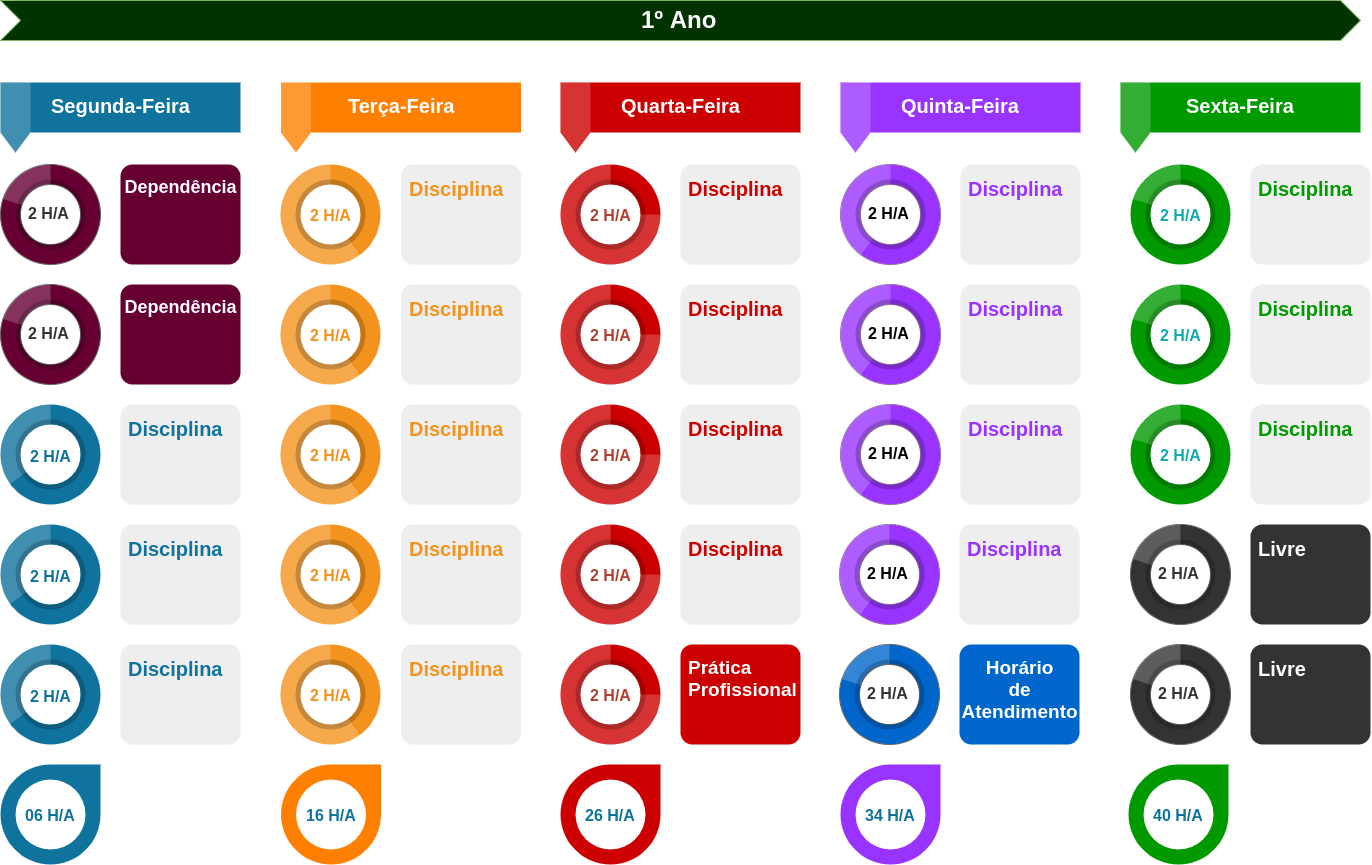
\includegraphics[width=.6\textwidth]{Alternativo01}
	\caption{Exemplo de distribuição da carga horária semanal no 1º Ano.}
	\label{fig:DiagramaSemanal01}
\end{figure}

\begin{figure}[!htp]
	\centering	
	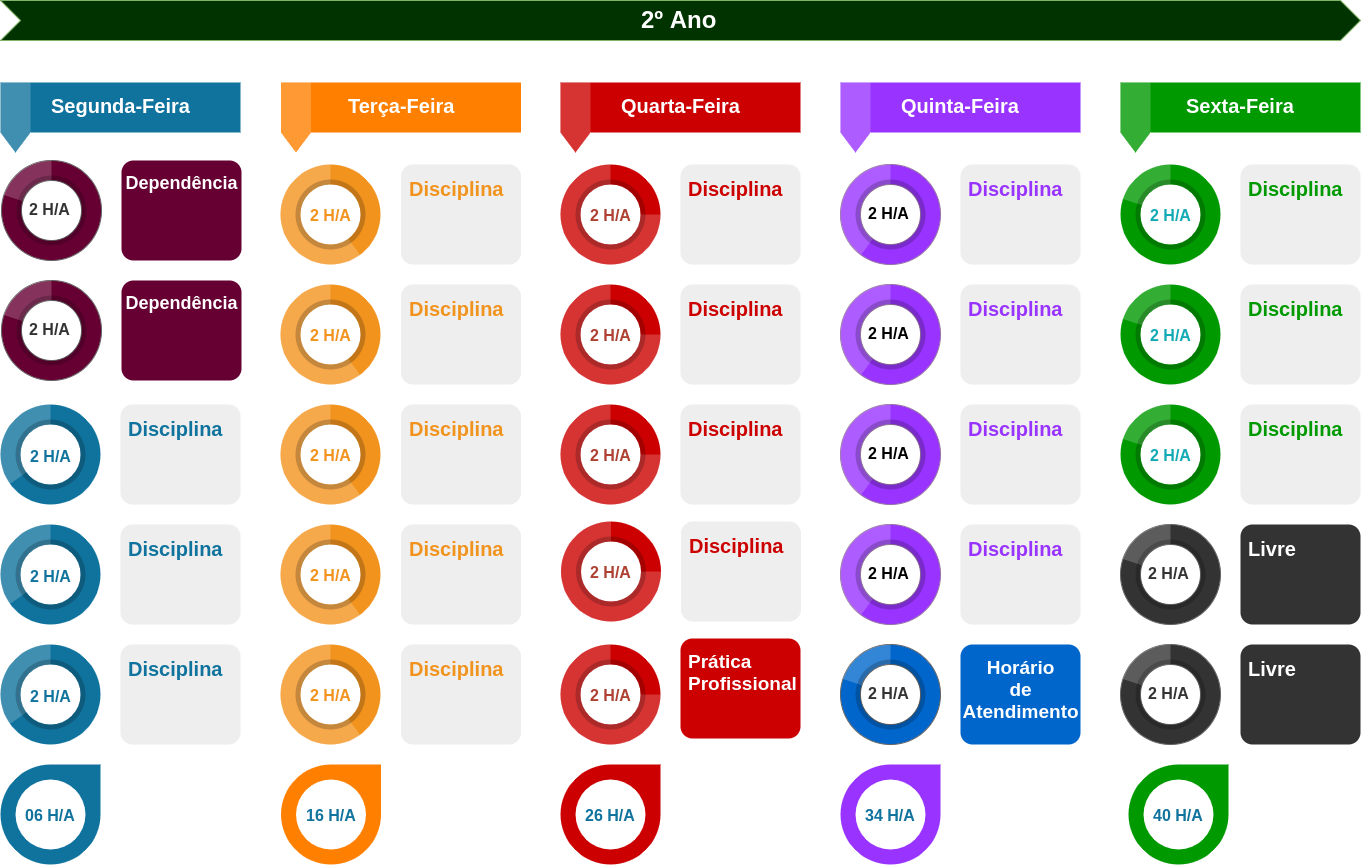
\includegraphics[width=.6\textwidth]{Alternativo02}
	\caption{Exemplo de distribuição da carga horária semanal no 2º Ano.}
	\label{fig:DiagramaSemanal02}
\end{figure}

\begin{figure}[!htp]
	\centering	
	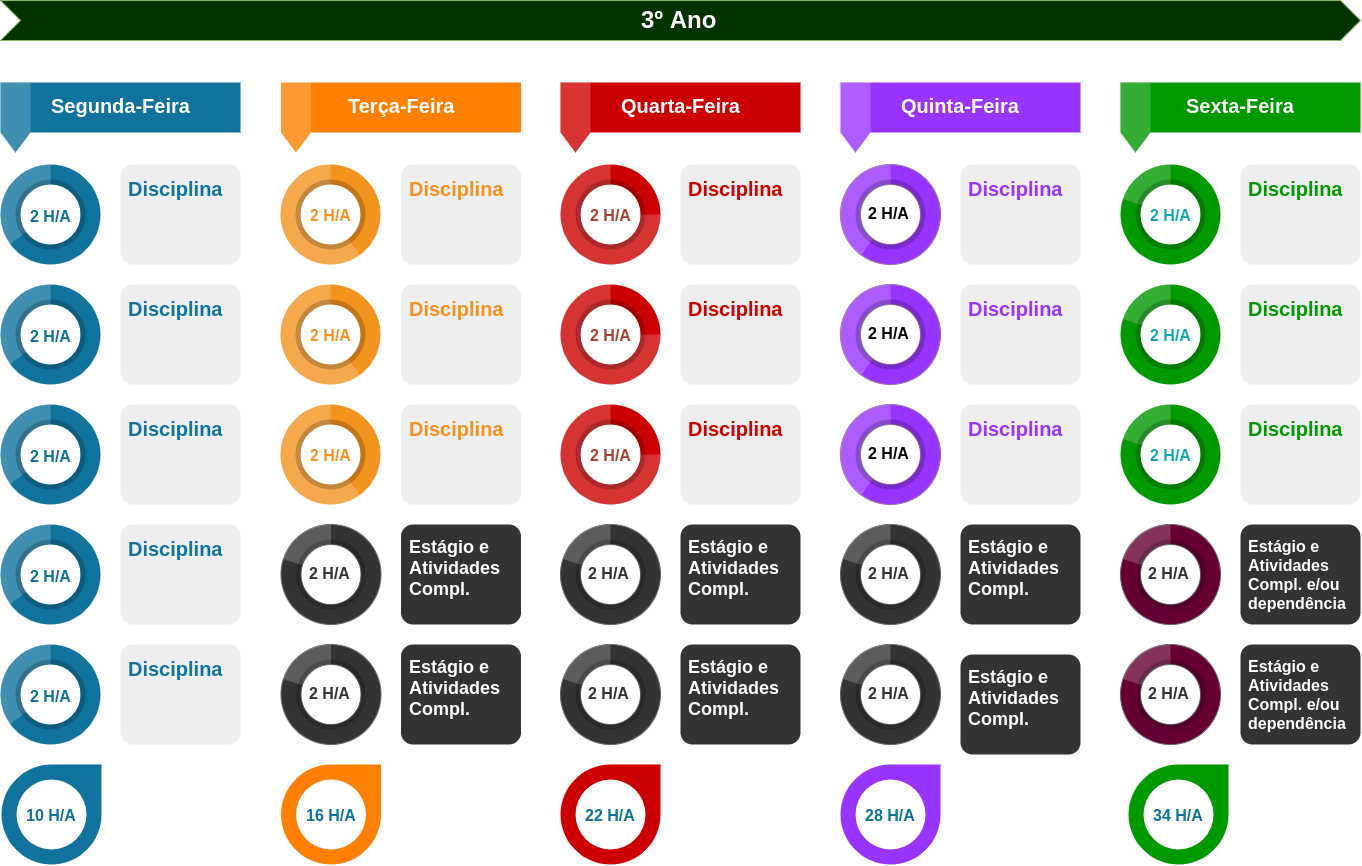
\includegraphics[width=.6\textwidth]{Alternativo03}
	\caption{Exemplo de distribuição da carga horária semanal no 3º Ano.}
	\label{fig:DiagramaSemanal03}
\end{figure}

\section{Metodologia de Ensino-Aprendizagem}\label{metodologia}
\indent

O Núcleo Politécnico foi desenhado para superar problemas clássicos que permeiam as práticas pedagógicas promovendo, juntamente com os núcleos Básico e Profissional, uma formação integral com vistas à indisssociabilidade da teoria e da prática, do ensino, da pesquisa e da extensão. 

Neste contexto, várias metodologias poderão ser aplicadas durante o período do curso, inclusive poderão partilhar dos princípios de metodologias ativas, como a estratégia pedagógica da problematização e de projetos, pois estas se complementam na tarefa de conduzir os participantes por um processo de aprendizagem significativa e suportada na participação ativa e crítico-reflexiva. 

\subsection{Prática Profissional}\label{praticasprofissionais}
\indent

Alicerçada no conhecimento e na inovação, e promovendo a aprendizagem colaborativa, a disciplina de prática profissional desenvolve nos estudantes a capacidade de trabalharem em equipe e aprenderemcom seus pares, além de estimular atitudes cooperativas e propositivas preparando-os para os desafios da comunidade, do mundo do trabalho e da sociedade em geral.

\begin{quote}
``\textit{A prática na Educação Profissional compreende diferentes situações de vivência, aprendizagem e trabalho, como experimentos e atividades específicas em ambientes especiais, tais como laboratórios, oficinas, empresas pedagógicas, ateliês e outros, bem como investigação sobre atividades profissionais, projetos de pesquisa e/ou intervenção, visitas técnicas, simulações, observações e outras}''~\cite{Resolucao06De2012}.
\end{quote}

Desta forma, o objetivo das Práticas Profissionais como disciplina atende simultaneamente à meta da BNCC, garantindo a contextualização dos conhecimentos, articulando as dimensões do trabalho, da ciência, da tecnologia e da cultura~\cite{BNCC2019} e à Resolução 06 de 20 de setembro de 2012, onde:
\begin{quote}
	\textit{A prática profissional, prevista na organização curricular do curso, deve estar continuamente relacionada aos seus fundamentos científicos e tecnológicos, orientada pela pesquisa como princípio pedagógico que possibilita ao educando enfrentar o desafio do desenvolvimento da aprendizagem permanente, integra as cargas horárias mínimas de cada habilitação profissional de técnico e correspondentes etapas de qualificação e de especialização profissional técnica de nível médio}~\cite{Resolucao06De2012}.
\end{quote}

A disciplina ~\ref{praticasprofissionais}, como componente curricular aloca um espaço de tempo destinado às diversas atividades técnico-científicas que podem ser desenvolvidas pelo estudante sob orientação docente, funcionando na prática como uma disciplina optativa de ementa aberta com no mínimo uma oferta anual no 1º e no 2º anos.
A disciplina poderá estar vinculada a Projetos de Ensino, de Extensão ou de Pesquisa.
Cada oferta contemplará um plano de atividades a serem desenvolvidas em ambientes especiais de ensino, tais como laboratórios, ateliês, oficinas, ginásios e outros, integrando a teoria com a prática e possibilitando a articulação com os organismos sociais, entre outros.

Práticas profissionais enquanto parte do processo de formação do estudante de cursos técnicos está presente como componente da matriz curricular com carga horária definida.
Como uma dimensão do processo ensino-aprendizagem, as práticas profissionais dialogam com a pesquisa e a extensão como princípios e métodos pedagógicos. 

\subsection{Atividades Complementares}\label{atividadescomplementares}
\indent

\begin{figure}[!htp]
	\centering	
	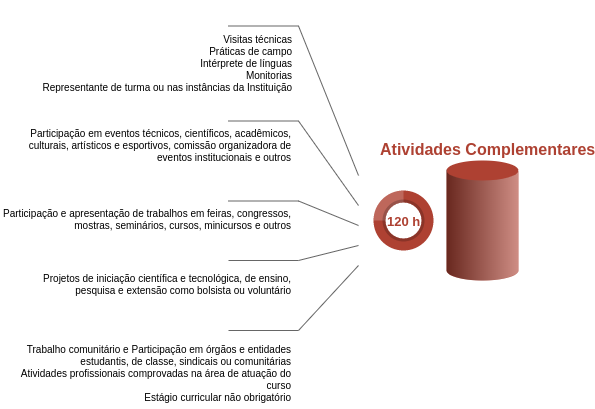
\includegraphics[width=.9\textwidth]{Pictures/AtividadesComplementares.png}
	\caption{Atividades que compõem as atividades complementares.}
	\label{fig:AtividadesComplementares}
\end{figure}

As atividades complementares serão cumpridas pelo aluno no período em que o mesmo estiver cursando as demais disciplinas da matriz curricular do curso, sendo um componente obrigatório para a conclusão do mesmo.
Elas ocorrerão, portanto, como parte integrante da matriz, respeitando a carga horária total mínima de 120 horas definida em regulamento~\cite{Resolucao20De2011}.
As integralização deste componente deverá obedecer aos dispostos no regulamento das Atividades Complementares dos cursos técnicos, aprovado pelo Conselho Superior da Instituição~\cite{Resolucao20De2011}.

\subsubsection{Estágio}
\indent

O Estágio Curricular é ato educativo escolar supervisionado, desenvolvido no ambiente de trabalho, que visa à preparação para o trabalho produtivo de educandos que estejam frequentando o ensino regular em instituições de educação superior, profissional, de ensino médio, da educação especial e dos anos finais do ensino fundamental na modalidade profissional da educação de jovens e adultos~\cite{Lei11788De2008}.

O Estágio Curricular deve promover a integração teórico/prático, aperfeiçoamento técnico cultural, científico e de relacionamento humano.  
Deve estimular ao aprendizado de competências próprias da atividade profissional, à efetiva integração entre ensino e serviço ou mundo do trabalho, à integração das atividades de estágio com as de ensino, pesquisa e outras ações de extensão, bem como à contextualização curricular, objetivando o desenvolvimento do educando para a vida cidadã e para o trabalho.

O Estágio Curricular supervisionado é caracterizado como prática profissional em situação real de trabalho e assumido como ato educativo. 
O discente poderá realizar estágio curricular obrigatório e não obrigatório. 
O estágio obrigatório é aquele definido na grade curricular deste PPC, cuja carga horária é requisito para aprovação e obtenção do diploma. 
Já o estágio não obrigatório é aquele desenvolvido como atividade opcional, em complementação à carga horária regular e obrigatória.

No Instituto Federal de Educação, Ciência e Tecnologia de Goiás (IFG), o estágio curricular no Curso Técnico em Biotecnologia Integrado ao Ensino Médio em Tempo Integral será obrigatório com carga horária total de 160 horas em acordo com a Resolução nº 22, de 26 de Dezembro de 2011~\cite{Resolucao22De2011}.
O estágio obedecerá ainda ao disposto na Lei nº 11.788, de 25 de Setembro de 2008~\cite{Lei11788De2008}, bem como as demais regulamentações e orientações emanadas pelos órgãos superiores competentes. 

As atividades a serem desenvolvidas no estágio devem estar em consonância com este documento e com as Regulamentações do Conselho Federal de Biologia, o Catálogo Nacional de Cursos Superiores de Tecnologia e demais legislações e regulamentações educacionais e profissionais vigentes.
Ainda, as atividades devem contribuir para que o estudante alcance o~\nameref{Perfil} descrito.

A formalização do Estágio, Obrigatório ou Não, deverá ser feita no IFG - Câmpus Formosa, observando-se os prazos estabelecidos nas resoluções institucionais vigentes.s
Para a realização e início das atividades do Estágio Curricular Obrigatório e Não Obrigatório, os seguintes requisitos devem ser atendidos pelo discente: estar regularmente matriculado no curso cuja área de atuação seja relacionada àquela em que a vaga de estágio está sendo pleiteada; ter cumprido mais de 50\% (cinquenta por cento) da carga horária do curso; firmar Termo de Compromisso de Estágio (TCE) entre as partes envolvidas no estágio (unidade concedente, IFG e discente), antes do início das atividades; ter o plano de atividades de estágio Curricular aprovado e assinado.

O TCE será firmado com duração máxima de 24 (vinte e quatro) meses na mesma parte concedente, exceto quando se tratar de estagiário portador de deficiência. 
O plano de atividades do estagiário, elaborado em acordo com as três partes envolvidas, unidade concedente, IFG e estagiário, será incorporado ao TCE por meio de aditivos à medida que for avaliado o desempenho do estudante. 
Quaisquer alterações no plano de atividades durante a execução do estágio devem ser respaldadas pela ciência tanto do supervisor quanto do professor orientador de estágio.
Em situações de mobilidade acadêmica, o estágio curricular obrigatório e não obrigatório, quando autorizado pela Coordenação do curso e Chefia do Departamento de Áreas Acadêmicas, poderá ser realizado sob a responsabilidade e orientação de outra instituição de educação, nacional ou estrangeira, mediante o pleno atendimento a este PPC e às normas acadêmicas e legais vigentes.

Os estudantes que realizam estágio fora do país dentro de programas de intercâmbio acadêmico obedecem aos procedimentos das instituições anfitriãs. 
Os estudantes que realizam estágio fora do país sem vínculo com outra instituição de ensino, ou seja, não estão em mobilidade acadêmica, obedecem aos procedimentos do IFG e devem ter o seu acompanhamento garantido pelas tecnologias disponíveis, assim não será necessário o procedimento de validação.

A jornada de atividades de estágio deve constar no TCE, sempre observando a compatibilidade com o horário escolar, não podendo ultrapassar os seguinte limite de 6 (seis) horas diárias e 30 (trinta) horas semanais. 
O estágio poderá ser realizado durante as férias ou recesso escolares, no mesmo período, ou no oposto ao que o estudante esteja matriculado, desde que tenha o acompanhamento de estágio garantido, podendo ser as atividades desempenhadas em unidades concedentes distintas.

O encerramento das atividades de Estágio Curricular ocorrerá compulsoriamente, após a data de encerramento prevista no TCE ou à pedido de qualquer uma das partes acordadas no TCE, desde que o pedido de rescisão seja devidamente formalizado por escrito.
Nos períodos de avaliação, a carga horária do estágio será reduzida pelo menos à metade, segundo estipulado no TCE, para garantir o bom desempenho do estudante. 
Não serão contabilizadas para integralização do estágio as horas não realizadas nos períodos de avaliação em que a carga horária tenha sido reduzida.
  
O acompanhamento do desenvolvimento do estágio pelos professores orientadores do IFG deverá ser realizado por uma das seguintes modalidades de supervisão acadêmica de estágio, supervisão indireta, semidireta e direta. 
A supervisão direta se caracteriza pelo acompanhamento e orientação das ações planejadas por observação contínua e direta das atividades ocorrentes nos campos de estágio ao longo de todo processo, podendo se complementar com entrevistas e reuniões, no âmbito do IFG e/ou no campo de estágio. 
Já a supervisão semidireta é caracterizada pelo acompanhamento e orientação das ações planejadas por meio de visitas sistemáticas ao campo de estágio pelo professor supervisor, que manterá também contatos com o profissional responsável pelo(s) estagiário(s), além do complemento de entrevistas e reuniões com os estudantes. 
Por fim, a supervisão indireta é o acompanhamento realizado via relatórios, reuniões ou visitas ocasionais aos campos de Estágio, onde deverão ocorrer reuniões com o profissional responsável.  

As atividades de estágio e as disciplinas e demais atividades curriculares de modalidade prática que necessitem de acompanhamento docente e da presença física do aluno em ambiente próprio, serão realizadas após o término do período de regime especial de exercício domiciliar e do consequente retorno do aluno às aulas.

As atribuições das partes envolvidas no processo de trabalho relacionado ao estágio, incluindo o IFG por meio dos setores responsáveis pelo estágio em nível de reitoria e dos câmpus, a unidade concedente de estágio, o estagiário, o coordenador do curso, o professor orientador e o supervisor de campo do estagiário da parte concedente, seguem as determinações do regulamento de estágio institucional em vigor.

\subsubsection{Atividades Não Presenciais e EaD}
\indent

Respeitados os mínimos previstos de duração e carga horária total, o plano de curso técnico de nível médio pode prever atividades não presenciais, até 20\% (vinte por cento) da carga horária diária do curso, desde que haja suporte tecnológico e seja garantido o atendimento por docentes e tutores~\cite{Resolucao06De2012}.

\subsubsection{Avaliação}

A avaliação, parte integrante do processo de aprendizagem, tem como objetivo o acompanhamento e a verificação de construção de competências por cada disciplina cursada pelo aluno.
Constitui-se num processo permanente e contínuo de análise do desempenho do aluno nas diferentes situações de aprendizagem, utilizando-se de um ou mais instrumentos usuais de avaliação, tais como: trabalhos de pesquisa; projetos interdisciplinares; resolução de situações-problema; apresentação de seminários; avaliação escrita ou oral; apresentação de artigos técnico/científico; relatórios; simulações e observação com roteiro e registros, bem como outras atividades que o docente julgar necessário.

Para fins de registro de desenvolvimento das competências, o resultado da avaliação deverá expressar o grau de desempenho de cada componente curricular, quantificado em nota de 0 (zero) a 10 (dez). 
Conforme estabelecido pela organização didática do IFG será considerando aprovado o aluno que obtiver média igual ou superior a 6,0 (seis) e frequência mínima obrigatória de 75\% da carga horária total da disciplina durante o ano letivo, conforme normatizado pela LDB~\cite{Lei19394De1996}.
A recuperação, quando necessária para suprir as eventuais dificuldades de aprendizagem, será aplicada paralelamente aos estudos ou ao final do semestre para correções indispensáveis e enriquecimento do processo de formação. 
O estudante poderá dar continuidade ao curso no semestre seguinte, mesmo ficando reprovado em até 03 componentes curriculares que não sejam pré-requisitos. 
Os critérios de avaliação das unidades curriculares atendem às normas vigentes na organização didática do IFG.


\section{Certificação}
\indent

Para obter o Certificado de Especialização em Ambiente, Ciência e Ensino do Cerrado, o discente deverá satisfazer as seguintes exigências:
\begin{itemize}
	\item Ser aprovado em todas as disciplinas do curso com nota mínima igual a 6,0 (sete) e freqüência igual ou superior a 75\% da carga horária da disciplina;
	\item Defender publicamente a monografia produzida perante uma Banca composta por, no mínimo, três professores (orientador, mais dois professores convidados, um externo e um interno ao campus IFG/Formosa) obtendo conceito Aprovado (AP);
	\item Possuir pelo menos um certificado que comprove a apresentação (pôster ou oral) de resultados relacionados à monografia exigida por essa pós-graduação em evento científico externo ao IFG (congressos, seminários, simpósios) cuja abrangência é, no mínimo, regional;
	\item Possuir documento (carta eletrônica ou impressa) que ateste a submissão em um periódico indexado de pelo menos um artigo produzido a partir dos resultados obtidos com o trabalho de conclusão de curso exigido por essa pós-graduação;
	\item Comprovar a quitação de suas obrigações junto à biblioteca do Campus Formosa do Instituto Federal de Educação, Ciência e Tecnologia de Goiás;
	\item Entregar toda a documentação exigida pelo processo seletivo.
\end{itemize}

O Certificado será emitido pelo Instituto Federal de Educação, Ciência e Tecnologia de Goiás, nos termos da Resolução CNE/CES n.º 1, de 8 de junho de 2007.	


\section{Dependências}
\indent

O IFG regulamenta a aprovação parcial por meio das dependências na Resolução nº 22, de 26 de Dezembro de 2011~\cite{Resolucao22De2011}.
Será admitida a aprovação parcial para a série seguinte, com dependência em até 02 (duas) disciplinas cabendo à Chefia de Departamento de Áreas Acadêmicas, por meio das coordenações acadêmicas, o acompanhamento do planejamento e realização das atividades e estudos de dependência no âmbito das disciplinas sob sua responsabilidade.
Cabe ainda ao Coordenador de Apoio Pedagógico ao Discente o acompanhamento dos discentes no cumprimento das atividades de dependência no âmbito dos cursos ofertados pelo respectivo Departamento~\cite{Resolucao22De2011}.

O aluno aprovado com dependência deverá cursá-la na série seguinte~\cite{Resolucao22De2011}.
Para o cumprimento das dependências curriculares o Departamento de Áreas Acadêmicas deverá assegurar atendimento docente ao aluno, fora do horário regular de aulas das disciplinas das respectivas turmas e cursos, sendo obrigatório o comparecimento do mesmo.
Nesse sentido há 8 horas/aula livres em contraturno diurno para realização das eventuais dependências por parte dos alunos.


%----------------------------------------------------------------------------------------
%	CHAPTER
%----------------------------------------------------------------------------------------
%------------------------------------------------
\chapterimage{04.jpg} % Chapter heading image
\chapter{Disciplinas e Ementas}
\vspace{6em}
\begin{flushright}
	\textit{\textcolor{white}{Foto: Adriano Darosci}}
\end{flushright}
\vspace{12em}

\section{Ementas do Núcleo Básico}\label{ementasBasico}
\indent

O núcleo básico comtempla os conhecimentos e as habilidades nas áreas de linguagens e códigos, ciências humanas, matemática e ciências da natureza, vinculados à Educação Básica (que) deverão permear o currículo dos cursos técnicos de nível médio, de acordo com as especificidades dos mesmos, como elementos essenciais para a formação e o desenvolvimento profissional do cidadão~\cite{Resolucao06De2012}.

As disciplinas aqui dispostas, visam viabilizar o acesso dos estudantes às bases científicas e tecnológicas dos processos de produção do mundo contemporâneo, relacionando teoria e prática – ou o conhecimento teórico à resolução de problemas da realidade social, cultural ou natural~\cite{BNCC2019}.

\newpage
\subsection{Artes}\label{disc:artes}
\begin{itemize}
	\item \textbf{Carga horária (hora/aula):} 108
	\item \textbf{Ementa 1º Ano:}
	Estudo sobre arte em suas linguagens, códigos e tecnologias específicas e suas influências culturais e educativas na sociedade;
	Conhecimento da arte como identidade, memória e criação, considerando suas expressões regionais e ressaltando as influências africanas e indígenas;
	Fundamentos, conceitos, funções, especificidades e características das artes visuais, dança, música, teatro e audiovisual;
	\item \textbf{Ementa 2º Ano:}
	Abordagens histórico-reflexivas das produções artístico-culturais da humanidade;
	Projetos de investigação e experimentação artística com técnicas, materiais, estilos e gêneros variados;
	Apreciação e compreensão de diferentes poéticas em diálogo com as manifestações artísticas regionais nas diversas linguagens;
	Estudo das matrizes culturais da arte brasileira, em especial as africanas e indígenas, a partir das diversas visões e versões de seus representantes;
	Relações entre arte e mundo do trabalho;
	\item \textbf{Bibliografia básica}
	\begin{enumerate}
		\item NNNNN
	\end{enumerate}
	\item \textbf{Bibliografia complementar}
	\begin{enumerate}
		\item 
	\end{enumerate}	
\end{itemize}
\nameref{tab:matriz}

\newpage
\subsection{Educação Física}\label{disc:educacaofisica}
\begin{itemize}
	\item \textbf{Carga horária (hora/aula):} 108
	\item \textbf{Ementa 1º Ano:} 
	Introdução ao estudo, vivência e reflexão crítica dos temas da cultura corporal de movimento, abordados pela Educação Física;
	Compreensão dos aspectos biológicos, históricos, psicológicos, sociais, filosóficos e culturais, e suas relações com o meio ambiente e a diversidade humana, em uma perspectiva omnilateral;
	
	\item \textbf{Ementa 2º Ano:} 
	Aprofundamento e ampliação do estudo, vivência e reflexão crítica dos temas da cultura corporal de movimento, abordados pela Educação Física;
	Educação Física e suas relações com o mundo do trabalho, a saúde e o lazer;	
	\item \textbf{Bibliografia básica}
	\begin{enumerate}
		\item NNNNN
	\end{enumerate}
	\item \textbf{Bibliografia complementar}
	\begin{enumerate}
		\item 
	\end{enumerate}	
\end{itemize}
\nameref{tab:matriz}

\newpage
\subsection{LIBRAS}\label{disc:libras}
\begin{itemize}
	\item \textbf{Carga horária (hora/aula):} 54
	\item \textbf{Ementa Espanhol:} 
	Estruturas básicas da Língua Espanhola em uma abordagem contrastiva com a Língua Portuguesa em seus aspectos lexicais, sintáticos, semânticos, pragmáticos, discursivos e interculturais; 
	Habilidades comunicativas de recepção e produção em vários gêneros textuais a partir das especificidades de cada curso;
	\item \textbf{Ementa LIBRAS:}
	Aspectos histórico-culturais do surdo. Noções básicas da gramática da Língua Brasileira de Sinais (LIBRAS);
	Vocabulário básico da LIBRAS;
	Práticas de conversação em LIBRAS;		
	\item \textbf{Bibliografia básica}
	\begin{enumerate}
		\item NNNNN
	\end{enumerate}
	\item \textbf{Bibliografia complementar}
	\begin{enumerate}
		\item 
	\end{enumerate}	
\end{itemize}
\nameref{tab:matriz}

\newpage
\subsection{Língua Estrangeira - Inglês}\label{disc:ingles}
\begin{itemize}
	\item \textbf{Carga horária (hora/aula):} 54
	\item \textbf{Ementa Inglês 2º Ano:} 
	Leitura, compreensão e interpretação de textos orais e escritos, estabelecendo relações entre língua, cultura e sociedade;
	Estudo de elementos morfossintáticos, semânticos e fonológicos da língua inglesa;
	Desenvolvimento das habilidades comunicativas com ênfase na leitura;
	Leitura, compreensão e interpretação de textos escritos, ligados à área de conhecimento do curso;
	\item \textbf{Bibliografia básica}
	\begin{enumerate}
		\item NNNNN
	\end{enumerate}
	\item \textbf{Bibliografia complementar}
	\begin{enumerate}
		\item 
	\end{enumerate}	
\end{itemize}
\VER{VER EMENTAS}
\nameref{tab:matriz}

\newpage
\subsection{Língua Estrangeira - Espanhol}\label{disc:espanhol}
\begin{itemize}
	\item \textbf{Carga horária (hora/aula):} 54
	\item \textbf{Ementa Espanhol 2º Ano:} 
	Estruturas básicas da Língua Espanhola em uma abordagem contrastiva com a Língua Portuguesa em seus aspectos lexicais, sintáticos, semânticos, pragmáticos, discursivos e interculturais; 
	Habilidades comunicativas de recepção e produção em vários gêneros textuais a partir das especificidades de cada curso;	
	\item \textbf{Bibliografia básica}
	\begin{enumerate}
		\item NNNNN
	\end{enumerate}
	\item \textbf{Bibliografia complementar}
	\begin{enumerate}
		\item 
	\end{enumerate}	
\end{itemize}
\VER{VER EMENTAS}
\nameref{tab:matriz}

\newpage
\subsection{Língua Estrangeira Opcional - Inglês ou Espanhol}\label{disc:ingles_espanhol}
\begin{itemize}
	\item \textbf{Carga horária (hora/aula):} 54
	\item \textbf{Ementa Inglês 3º Ano:} 
	Leitura, compreensão e interpretação de textos orais e escritos, estabelecendo relações entre língua, cultura e sociedade;
	Estudo de elementos morfossintáticos, semânticos e fonológicos da língua inglesa;
	Desenvolvimento das habilidades comunicativas com ênfase na leitura;
	Leitura, compreensão e interpretação de textos escritos, ligados à área de conhecimento do curso;
	\item \textbf{Ementa Espanhol 3º Ano:} 
	Estruturas básicas da Língua Espanhola em uma abordagem contrastiva com a Língua Portuguesa em seus aspectos lexicais, sintáticos, semânticos, pragmáticos, discursivos e interculturais; 
	Habilidades comunicativas de recepção e produção em vários gêneros textuais a partir das especificidades de cada curso;	
	\item \textbf{Bibliografia básica}
	\begin{enumerate}
		\item NNNNN
	\end{enumerate}
	\item \textbf{Bibliografia complementar}
	\begin{enumerate}
		\item 
	\end{enumerate}	
\end{itemize}
\VER{VER EMENTAS}
\nameref{tab:matriz}


\newpage
\subsection{Língua Portuguesa, Leitura e Produção de Textos}\label{disc:linguaportuguesa}
\begin{itemize}
	\item \textbf{Carga horária (hora/aula):} 270
%	\item \textbf{Conceitos-Chave:}
%	\begin{itemize}
%		\item Interpretação de textos técnicos
%		\item Redação de textos técnicos
%	\end{itemize}
	\item \textbf{Ementa 1º Ano:} 
	Práticas de leitura, compreensão, interpretação e produção de textos de diversos gêneros textuais
	Análise linguística: integração dos níveis morfossintático e discursivo;
	Literatura brasileira e seus aspectos estilísticos e culturais em diálogo com a cultura afro-brasileira e indígena;
	Usos da Língua em diferentes registros e níveis de formalidade;

	\item \textbf{Ementa 2º Ano:} 
	Práticas de leitura, compreensão, interpretação e produção de textos de diversos gêneros textuais
	Análise linguística: integração dos níveis morfossintático e discursivo;
	Literatura brasileira e seus aspectos estilísticos e culturais em diálogo com a cultura afro-brasileira e indígena;
	Usos da Língua em diferentes registros e níveis de formalidade;

	\item \textbf{Ementa 3º Ano:} 
	Práticas de leitura, compreensão, interpretação e produção de textos de diversos gêneros textuais
	Análise linguística: integração dos níveis morfossintático e discursivo;
	Literatura brasileira e seus aspectos estilísticos e culturais em diálogo com a cultura afro-brasileira e indígena;
	Usos da Língua em diferentes registros e níveis de formalidade;	
	
	\item \textbf{Bibliografia básica}
	\begin{enumerate}
		\item NNNNN
	\end{enumerate}
	\item \textbf{Bibliografia complementar}
	\begin{enumerate}
		\item 
	\end{enumerate}	
\end{itemize}
\VER{VER EMENTAS}
\nameref{tab:matriz}

\newpage
\subsection{Matemática}\label{disc:matematica}
\begin{itemize}
	\item \textbf{Carga horária (hora/aula):} 270
	\item \textbf{Ementa 1º Ano:} 4 horas-sula semanais\\
	Conjuntos;
	Funções: introdução, afim, quadrática, modular, exponencial e logarítmica;
	Progressão aritmética;
	Progressão geométrica;
	Noções de Estatística;
	
	\item \textbf{Ementa 2º Ano:} 4 horas-sula semanais\\
	Trigonometria;
	Funções trigonométricas;
	Geometria plana e espacial;
	Sistemas lineares;
	Matrizes;
	Determinantes;
	Análise Combinatória;
	Probabilidade;
		
	\item \textbf{Ementa 3º Ano:} 2 horas-sula semanais\\
	Geometria analítica; 
	Equações polinomiais; 
	Números complexos; 
	Conceitos básicos de Bioestatística, tais como: organização dos dados quantitativos;
	Medidas de tendência central e de dispersão; distribuições; formulação de testes de hipóteses; 
	Médias e correlações;
	

	\item \textbf{Bibliografia básica}
	\begin{enumerate}
		\item NNNNN
	\end{enumerate}
	\item \textbf{Bibliografia complementar}
	\begin{enumerate}
		\item 
	\end{enumerate}	
\end{itemize}
\nameref{tab:matriz}

\newpage
\subsection{Geografia}\label{disc:geografia}
\begin{itemize}
	\item \textbf{Carga horária (hora/aula):} 162
	\item \textbf{Ementa 1º Ano:} 
	A contribuição da Geografia para compreensão da realidade/mundo;
	Formas de representação espacial;
	A dinâmica da natureza e as interfaces com a formação das paisagens;
	Apropriação da natureza pelo trabalho e a questão ambiental;
	\item \textbf{Ementa 2º Ano:} 	
	Constituição do território brasileiro;
	Formação das identidades no Brasil; 
	Dinâmica da natureza e a paisagem brasileira;
	Desenvolvimento industrial e urbanização no Brasil;
	Ocupação produtiva e a agricultura no Brasil; 
	Dinâmica demográfica e relações étnico-culturais no Brasil;
	Geografia de Goiás;
	\item \textbf{Ementa 3º Ano:} 	
	Espacialização das relações capitalistas de produção e a sociedade em rede;
	O processo de urbanização e a questão campo/cidade;
	Dinâmica demográfica e as relações étnico-culturais mundiais;
	Regionalização do espaço mundial e as novas modalidades de exclusão;
	Território, conflitos e geopolítica mundial;
	\item \textbf{Bibliografia básica}
	\begin{enumerate}
		\item NNNNN
	\end{enumerate}
	\item \textbf{Bibliografia complementar}
	\begin{enumerate}
		\item 
	\end{enumerate}	
\end{itemize}
\nameref{tab:matriz}

\newpage
\subsection{História}\label{disc:historia}
\begin{itemize}
	\item \textbf{Carga horária (hora/aula):} 162
	\item \textbf{Ementa 1º Ano:} 
	Estudos históricos em relações entre trabalho, produção, tecnologia, ciência, meio ambiente, questões étnico-culturais, de gênero, memória e as articulações destes elementos no interior de cada formação social, articulando o global e o local, bem como suas implicações nas diversas realidades; 
	Análise de processos de transformações/permanências/ resistências/semelhanças e diferenças nas dimensões políticas, econômicas, sociais e culturais;
	Sociedades ágrafas, antigas e medievais;
	\item \textbf{Ementa 2º Ano:} 
	Estudos históricos em relações entre trabalho, produção, tecnologia, ciência, meio ambiente, questões étnico-culturais, de gênero, memória e as articulações destes elementos no interior de cada formação social, articulando o global e o local, bem como suas implicações nas diversas realidades; 
    Análise de processos de transformações/permanências/ resistências/semelhanças e diferenças nas dimensões políticas, econômicas, sociais e culturais;		
	Construção do mundo moderno: Europa, Ásia, Áfricas, Américas;
	Processos revolucionários dos séculos XVIII e XIX; 
	Brasil Império;
	\item \textbf{Ementa 3º Ano:} 
	Estudos históricos em relações entre trabalho, produção, tecnologia, ciência, meio ambiente, questões étnico-culturais, de gênero, memória e as articulações destes elementos no interior de cada formação social, articulando o global e o local, bem como suas implicações nas diversas realidades; 
	Análise de processos de transformações/permanências/ resistências/semelhanças e diferenças nas dimensões políticas, econômicas, sociais e culturais;			
	Construção do mundo contemporâneo: do imperialismo à globalização; 
	Brasil República;
	\item \textbf{Bibliografia básica}
	\begin{enumerate}
		\item NNNNN
	\end{enumerate}
	\item \textbf{Bibliografia complementar}
	\begin{enumerate}
		\item 
	\end{enumerate}	
\end{itemize}
\nameref{tab:matriz}

\newpage
\subsection{Física}\label{disc:fisica}
\begin{itemize}
	\item \textbf{Carga horária (hora/aula):} 162
	\item \textbf{Ementa 1º Ano:} 
	Movimentos: variações e conservações;
	\item \textbf{Ementa 2º Ano:}	
	Calor, ambiente e uso de energia;
	Som, imagem e informação;
	\item \textbf{Ementa 3º Ano:}	
	Equipamentos elétricos e telecomunicações;
	Matéria e radiação: 
	Noções de radioatividade;
	\item \textbf{Bibliografia básica}
	\begin{enumerate}
		\item NNNNN
	\end{enumerate}
	\item \textbf{Bibliografia complementar}
	\begin{enumerate}
		\item 
	\end{enumerate}	
\end{itemize}
\nameref{tab:matriz}

\newpage
\subsection{Filosofia}\label{disc:filosofia}
\begin{itemize}
	\item \textbf{Carga horária (hora/aula):} 162
	\item \textbf{Ementa 1º Ano:} 
	Introdução à filosofia e ao filosofar;
	Elementos conceituais da teoria do conhecimento, da ontologia e das estruturas do pensamento e da linguagem;
	%\VER{Abordagem da ética filosófica à ética aplicada em saúde;}\footnote{Veio de~\nameref{disc:bioeticalab}} 
	\item \textbf{Ementa 2º Ano:} 	
	Fundamentos, concepções e relações da ética e da política; 
	Valores, direitos humanos, liberdade e virtude;
	\sout{Estado, poder, soberania, ideologia e formas de governo;}\footnote{Vai para~\nameref{disc:sociologia}}
	\item \textbf{Ementa 3º Ano:} 
	Fundamentos conceituais da ciência, da subjetividade e da estética;
	O significado e as implicações dos processos científicos e da técnica; 
	A crise da razão;
	\item \textbf{Bibliografia básica}
	\begin{enumerate}
		\item NNNNN
	\end{enumerate}
	\item \textbf{Bibliografia complementar}
	\begin{enumerate}
		\item 
	\end{enumerate}	
\end{itemize}
\nameref{tab:matriz}

\newpage
\subsection{Sociologia}\label{disc:sociologia}
\begin{itemize}
	\item \textbf{Carga horária (hora/aula):} 162
	\item \textbf{Ementa 1º Ano:} 
	A Sociologia como ciência e sua origem; 
	Indivíduo e sociedade; 
	Instituições sociais; 
	Correntes clássicas do pensamento sociológico; 
	Modernidade e capitalismo;
	\item \textbf{Ementa 2º Ano:} 
	Cultura, etnocentrismo, relativismo cultural e diversidade: relações étnico-raciais, gênero, geração, sexualidade;
	Educação e sociedade; 
	Desigualdades sociais; 
	Trabalho e organização produtiva; 
	Globalização e Mundialização do do capital; 
	Indústria cultural e consumo;
	\item \textbf{Ementa 3º Ano:} 
	\VER{	
	Estado, ideologia e regimes políticos; 
	Sistemas de governo;
	}\footnote{Veio de~\nameref{disc:filosofia}} 
	Movimentos sociais;
	Cidadania e participação social;
	Política;
	\item \textbf{Bibliografia básica}
	\begin{enumerate}
		\item NNNNN
	\end{enumerate}
	\item \textbf{Bibliografia complementar}
	\begin{enumerate}
		\item 
	\end{enumerate}	
\end{itemize}
\nameref{tab:matriz}

\newpage
\section{Ementas do Núcleo Politécnico}\label{ementasPolitecnico}
\indent

O núcleo politécnico compreende os fundamentos científicos, sociais, organizacionais, econômicos, políticos, culturais, ambientais, estéticos e éticos que alicerçam as tecnologias e a contextualização do mesmo no sistema de produção social de forma aderenta ao eixo tecnológico em que se situa o curso~\cite{Resolucao06De2012}.


\newpage
\subsection{Química Geral}\label{disc:quimica}
\begin{itemize}
	\item \textbf{Carga horária (hora/aula):} 108
	\item \textbf{Conceitos-Chave:}
	\begin{itemize}
		\item NNNNN
		\item NNNNN
	\end{itemize}
	\item \textbf{Ementa 1º Ano:}
	\begin{itemize}	
		\item \textbf{Ementa:} 
		%Leis ponderais;
		Matéria, energia, transformações, substâncias;
		Modelos e estrutura atômica;
		Tabela periódica;
		Ligações e interações químicas;
		Funções inorgânicas;
		Reações químicas;
		Noções de radioatividade;
		Equilíbrio em meio homogêneo (Ácido - Base): teoria ácido-base (segundo Arhenius, Brönsted e Lewis);
		Equilíbrio químico;
	\end{itemize}
	%Parte de fisico-quimica ficou junto com quimica analitica
	\item \textbf{Bibliografia básica}
	\begin{enumerate}
		\item NNNNN
	\end{enumerate}
	\item \textbf{Bibliografia complementar}
	\begin{enumerate}
		\item 
	\end{enumerate}	
\end{itemize}
\nameref{tab:matriz}


\newpage
\subsection{Química Orgânica}\label{disc:quimica_organica}
\begin{itemize}
	\item \textbf{Carga horária (hora/aula):} 54
	\item \textbf{Conceitos-Chave:}
	\begin{itemize}
		\item NNNNN
		\item NNNNN
	\end{itemize}
	\item \textbf{Ementa 1º Ano:}
	\begin{itemize}	
		\item \textbf{Ementa:} 
		Introdução à química orgânica;
		
		Funções orgânicas: hidrocarbonetos, oxigenadas e nitrogenadas, e suas principais reações; 

		Isomeria;
	\end{itemize}
	%Parte de fisico-quimica ficou junto com quimica analitica
	\item \textbf{Bibliografia básica}
	\begin{enumerate}
		\item NNNNN
	\end{enumerate}
	\item \textbf{Bibliografia complementar}
	\begin{enumerate}
		\item 
	\end{enumerate}	
\end{itemize}
\nameref{tab:matriz}

\newpage
\subsection{Biologia}\label{disc:biologia}
\begin{itemize}
	\item \textbf{Carga horária (hora/aula):} 108
%	\item \textbf{Conceitos-Chave:}
%	\begin{itemize}
%		\item Interações entre organismos e entre organismos e o meio ambiente.
%		\item Origem, particularidades e conservação da Biodiversidade.
%	\end{itemize}
	\item \textbf{Ementa 1º Ano:}
	\begin{itemize}
		\item \textbf{Ementa 1º Semestre:} 
		Célula: histórico, tipos, componentes e funcionamento; 
		Reprodução sexuada e assexuada; 
		Ciclos de vida; 
		Seres vivos: Classificação, organização e importância econômica e ambiental; 
		Anatomia e histologia animal;
		Embriogênese.
%		Seres vivos: Classificação, organização e importância econômica e ambiental;
%		Ciclos Biogeoquímicos; 
%		Célula: teoria, padrões e componentes; 
%		Divisão celular;
%		Morfologia e fisiologia humana;
		
		\item \textbf{Ementa 2º Semestre:} 
		Origem da vida; 
		Teorias e mecanismos evolutivos; 
		Ecologia: população, comunidades e ecossistemas; 
		Ciclos Biogeoquímicos; 
		Métodos sustentáveis de produção.
%		Origem da vida; 
%		Teorias e mecanismos evolutivos;
%		Ecologia: Conceitos básicos, ecologia de população, comunidades e ecossistemas; 
%		Poluição e sustentabilidade;
		\end{itemize}
	\item \textbf{Bibliografia básica}
	\begin{enumerate}
		\item CAMPBELL, Neil A. et al. Biologia. 8. ed. Porto Alegre: Artmed, 2010.
		\item SADAVA, David et al. Vida: a ciência da biologia, 2: evolução, diversidade e ecologia. 8. ed.Porto Alegre: Artmed, 2009.
		\item SADAVA, David E. Vida: a ciência da biologia: célula e hereditariedade. Vol. 1. 8ª Ed. Porto Alegre: Artmed, 2009.
	\end{enumerate}
	\item \textbf{Bibliografia complementar}
	\begin{enumerate}
		\item BIZZO, Nelio Marco Vincenzo. Novas bases da biologia: seres vivos e comunidades. Vol. 2. São Paulo: Ática, 2011.
		\item LINHARES, Sérgio de Vasconcellos. Biologia hoje. Vol. 2. 12ª Ed. São Paulo: Ática, 2009.
		\item MARGULIS, Lynn; SCWARTZ, Karlene V. Cinco reinos: um guia  ilustrado dos filos da vida na Terra. 3. ed. Rio de Janeiro: Guanabara Koogan, 2009.
		\item PAULINO, Wilson Roberto. Biologia. Vol. 1, 2 e 3. 16ª Ed. São Paulo: Ática, 2007.
		\item SILVA-JÚNIOR, César da. Biologia: volume único. 4. Ed. São Paulo: Saraiva, 2007.
	\end{enumerate}	
\end{itemize}
\nameref{tab:matriz}



\newpage
\subsection{Bioquímica}\label{disc:bioquimica}
\begin{itemize}
	\item \textbf{Carga horária (hora/aula):} 54
	\item \textbf{Ementa:}
	Introdução à Bioquímica; 
	
	Biomoléculas e nutrientes;
	
	Reações de biossíntese e degradação;
	
	Metabolismo e aplicações de carboidratos, lipídios e proteínas;
	
	Princípios de bioenergética;

	\item \textbf{Bibliografia básica}
	\begin{enumerate}
		\item NNNNN
	\end{enumerate}
	\item \textbf{Bibliografia complementar}
	\begin{enumerate}
		\item 
	\end{enumerate}	
\end{itemize}
\nameref{tab:matriz}


\newpage
\subsection{Biologia Molecular e Genética}\label{disc:biomol}
\begin{itemize}
	\item \textbf{Carga horária (hora/aula):} 108
	\item \textbf{Ementa:}
	Dogma central da Biologia Molecular e o fluxo da informação genética;
	
	Estrutura, propriedades e características de ácidos nucléicos (DNA e RNA);

	Histonas e empacotamento do DNA eucariótico; 	
	
	Replicação e transcrição em procariotos e eucariotos;
	
	Mecanismo de processamento do mRNA eucariótico; 
	
	Tradução, código genético e processos traducionais; 
	
	%Amplificação gênica \textit{in vivo} e \textit{in vitro}; 
	
	Reparo e mutagênese;
	
	Introdução à Genética;

	Probabilidade e teste de proporções genéticas; 

	Mendelismo: os princípios básicos da herança; 

	Extensões do mendelismo; 

	Genes ligados ao sexo em seres humanos;

	Genética quantitativa: modelos para cor da pele humana e discussão das questões étnico-raciais à luz da genética moderna;

	Variação no número e estrutura dos cromossomos;

	Técnicas básicas de Biologia Molecular e manipulação genética;
	
	\item \textbf{Bibliografia básica}
	\begin{enumerate}
		\item NNNNN
	\end{enumerate}
	\item \textbf{Bibliografia complementar}
	\begin{enumerate}
		\item 
	\end{enumerate}	
\end{itemize}
\nameref{tab:matriz}

\newpage
\subsection{Bioética}\label{disc:bioetica}
\begin{itemize}
	\item \textbf{Carga horária (hora/aula):} 54
	\item \textbf{Ementa:} 
	\sout{Abordagem da ética filosófica à ética aplicada em saúde;}\footnote{Foi para~\nameref{disc:filosofia}}
	
	Princípios e teorias da bioética;
	
	Produção de conhecimento e o exercício profissional em biotecnologia; 
	
	Papel e limites das ciências e do cientista; 
	
	Discussão de questões teóricas voltadas a questões da bioética constitutivas dos campos das relações emergentes e das relações persistentes de nossa sociedade; 
	
	Bioética e a saúde pública, eutanásia e distanásia, segurança alimentar; 
	
	Transgênicos; 
	
	Especismo; 
	
	Tecnologias emergentes;
	
	Bioterrorismo; 
	
	Aborto;
	
	Direitos humanos;
	\item \textbf{Bibliografia básica}
	\begin{enumerate}
		\item NNNNN
	\end{enumerate}
	\item \textbf{Bibliografia complementar}
	\begin{enumerate}
		\item 
	\end{enumerate}	
\end{itemize}
\nameref{tab:matriz}

\newpage
\subsection{Fundamentos de Laboratório, Biossegurança e Inovação}\label{disc:bioseg}
\begin{itemize}
	\item \textbf{Carga horária (hora/aula):} 54
	\item \textbf{Ementa:} 
	Conceito de Biossegurança e sua importância; 
	
	Legislação, normas e medidas de biossegurança nas atividades desenvolvidas pelos profissionais de biotecnologia; 
	
	Riscos químicos, físicos e biológicos;
	
	Condutas de segurança e saúde no trabalho; 
	
	Transporte e descarte dos resíduos de serviço de saúde e relação com o meio ambiente; 
	
	Noções de metodologia científica;
	
	Elaboração de projetos de pesquisa; 
	
	Propriedade intelectual: conceitos e modalidades;
	
	Gestão da propriedade intelectual;
	
	Gestão da inovação e transferência de tecnologia;
	
	Prospecção tecnológica;
	
	Noções de empreendedorismo;	
	\item \textbf{Bibliografia básica}
	\begin{enumerate}
		\item NNNNN
	\end{enumerate}
	\item \textbf{Bibliografia complementar}
	\begin{enumerate}
		\item 
	\end{enumerate}	
\end{itemize}
\nameref{tab:matriz}

\newpage
\subsection{Estudo Orientado e Prática profissional}\label{disc:pratica}
\indent
\begin{itemize}
	\item \textbf{Carga horária (hora/aula):} 216
	\item \textbf{Ementa:} Momento presencial com carga horária de 2 horas semanais para prática na Educação Profissional nos termos da Resolução 06/2012~\cite{Resolucao06De2012}.
	\item \textbf{Bibliografia básica}
	\begin{enumerate}
		\item NNNNN
	\end{enumerate}
	\item \textbf{Bibliografia complementar}
	\begin{enumerate}
		\item 
	\end{enumerate}	
\end{itemize}
\nameref{tab:matriz}

\newpage
\section{Ementas do Núcleo Profissional}\label{ementasTecnico}
\indent

O núcleo profissional contempla métodos, técnicas, ferramentas e outros elementos das tecnologias relativas aos cursos~\cite{Resolucao06De2012}.

\newpage
\subsection{Biotecnologia Animal}\label{disc:biotecAnimal}
\begin{itemize}
	\item \textbf{Carga horária (hora/aula):} 54
	\item \textbf{Ementa:}	
	Zoologia: classificação, organização e fisiologia;
	
	Fundamentos de regulação homeostática, nutrição, digestão, metabolismo, osmorregulação e excreção, ventilação e circulação, músculo e movimento;
	
	Reprodução; 

	Regulação neuroendócrina; coordenação e interação dos organismos animais; evolução e filogênese do sistema nervoso; 
	
	Sistema sensorial e motor de invertebrados e vertebrados;	
	
	Técnicas de controle de pragas \textit{in vivo} e \textit{in vitro};
	
	Biotecnologia Animal no Brasil e no mundo; 
	
	Situação atual e perspectivas.
	\item \textbf{Bibliografia básica}
	\begin{enumerate}
		\item NNNNN
	\end{enumerate}
	\item \textbf{Bibliografia complementar}
	\begin{enumerate}
		\item 
	\end{enumerate}	
\end{itemize}
\nameref{tab:matriz}

\newpage
\subsection{Biotecnologia Vegetal}\label{disc:biotecVegetal}
\begin{itemize}
	\item \textbf{Carga horária (hora/aula):} 54
	\item \textbf{Ementa:}	
	Morfologia básica e tipos de raiz, caule, folha, flor e fruto; 
	
	Crescimento primário e secundário em raízes e caules; 
	
	Principais tecidos da folha;	

	Fotossíntese; 
	
	Hormônios Vegetais; 
	
	Processos básicos da fisiologia vegetal; 
	
	Principais técnicas da biotecnologia vegetal.
	\item \textbf{Bibliografia básica}
	\begin{enumerate}
		\item FERRI, Mário Guimarães. Fisiologia vegetal, 1. 2. ed. São Paulo: EPU, 2004. 
		\item PRADO, Carlos Henrique B. de A.; CASALI, Carlos Aparecido.  Fisiologia vegetal: práticas em relações hídricas, fotossíntese e nutrição mineral. Barueri: Manole, 2006.
		\item TAIZ, Lincoln; ZEIGER, Eduardo. Fisiologia vegetal. 4. ed. Porto Alegre: Artmed, 2010.
	\end{enumerate}
	\item \textbf{Bibliografia complementar}
	\begin{enumerate}
		\item ESAU, Katherine. Anatomia das plantas com sementes. São Paulo: Bluch;
		\item MARENCO, R. A. Fisiologia vegetal: fotossíntese, respiração, relações mineral. 3 ed. Viçosa: Universidade Federal de Viçosa. 2011;
		\item CAMPBELL, Neil A. et al. Biologia. 8. ed. Porto Alegre: Artmed, 2010;
		\item RAVEN, Peter H.; EVERT, Ray F.; EICHHORN, Susan E. Biologia vegetal. 7. ed. Rio de Janeiro: Guanabara Koogan, 2010;
		\item SADAVA, David et al. Vida: a ciência da biologia, 2: evolução, diversidade e ecologia. 8. ed.Porto Alegre: Artmed, 2009.
	\end{enumerate}	
\end{itemize}
\nameref{tab:matriz}

\newpage
\subsection{Físico Química e Química Analítica}\label{disc:analitica}
\begin{itemize}
	\item \textbf{Carga horária (hora/aula):} 108
	
	Estequiometria; Soluções e propriedades coligativas; 
	
	Eletroquímica;
	
	Termoquímica; Cinética química; 
	
	Introdução ao Estudo de Química Analítica: marcha geral de análise, seletividade e especificidade, sensibilidade ou limite de detecção; 
	
	Reações Redox; 
	
	Método gráfico para determinação e especiação das espécies químicas estudadas;
	
	Análise sistemática x Análise assistemática: análise de cátions;
	
	Métodos quantitativos; Amostragem; 
	
	Medição em química analítica; 
	
	Material volumétrico e balança analítica; Introdução à análise volumétrica; 
	
	Volumetria de neutralização; 
	
	Análise gravimétrica; 
	
	Volumetria de oxidação-redução; 
	
	Volumetria de precipitação; 
	
	Potenciometria; 
	
	Absorção atômica;
	\item \textbf{Bibliografia básica}
	\begin{enumerate}
		\item NNNNN
	\end{enumerate}
	\item \textbf{Bibliografia complementar}
	\begin{enumerate}
		\item 
	\end{enumerate}	
\end{itemize}
\nameref{tab:matriz}

%\newpage
%\subsection{Biotecnologia de Alimentos}\label{disc:biotecAlimentos}
%\begin{itemize}
%	\item \textbf{Carga horária (hora/aula):} 54
%	\item \textbf{Ementa 1º semestre:}	
%	Introdução aos princípios e processos tecnológicos envolvidos no processamento de alimentos;
%	Estudos das modificações bioquímicas dos alimentos durante o desenvolvimento, armazenamento e processamento;
%	Fundamentos da produção biotecnológica para o desenvolvimento de produtos e processos alimentícios (carnes, laticínios, cereais vegetais, ovo, pães, aditivos e derivados);
%	\item \textbf{Ementa 2º semestre:}	
%	Boas práticas de manufatura;
%	Análise de risco e pontos críticos de controle;
%	Conservação de alimentos;
%	Embalagens;
%	Bioquímica e bromatologia de alimentos;
%	\item \textbf{Bibliografia básica}
%	\begin{enumerate}
%		\item NNNNN
%	\end{enumerate}
%	\item \textbf{Bibliografia complementar}
%	\begin{enumerate}
%		\item 
%	\end{enumerate}	
%\end{itemize}
%\nameref{tab:matriz}

\newpage
\subsection{Biotecnologia e Saúde Humana}\label{disc:biotecSaude}
\begin{itemize}
	\item \textbf{Carga horária (hora/aula):} 54
	
	Relação dos parasitos e seus efeitos no sistema imune do hospedeiro; 
	
	Identificação dos parasitos que acometem o homem e alguns os animais domésticos: protozoologia, helmintologia, entomologia e acarologia, as formas de transmissão e diagnósticos laboratoriais; 
	
	\VER{Fatores sanguíneos}
	
	Epidemiologia e profilaxia; 
	
	Estudo dos mecanismos da resposta imune inata e adaptativa; 
	
	Reconhecimento de antígenos; 
	
	Maturação, ativação e regulação dos linfócitos;
	
	Mecanismos efetores envolvidos na resposta imune;
	
	Processos patológicos decorrentes de alterações nos mecanismos normais de resposta imunológica;
	
	\VER{Vacinas, antibióticos, antifúngicos, hormônios, interferons, interleucinas, anticorpos monoclonais;}
	
	\item \textbf{Bibliografia básica}
	\begin{enumerate}
		\item NNNNN
	\end{enumerate}
	\item \textbf{Bibliografia complementar}
	\begin{enumerate}
		\item 
	\end{enumerate}	
\end{itemize}
\nameref{tab:matriz}


\newpage
\subsection{Microbiologia Aplicada à Biotecnologia}\label{disc:microbiologia}
\begin{itemize}
	\item \textbf{Carga horária (hora/aula):} 108
	
	Introdução e histórico da microbiologia; 
	
	Microrganismos: classificação, citologia, morfologia, metabolismo, crescimento, controle do crescimento, genética e técnicas microbiológicas básicas;
	
	Cinética de crescimento microbiano;
	
	Microbiologia industrial; 
	
	Principais microrganismos e bioprodutos industriais: produção, melhoramento e características gerais;
	
	\VER{Noções de bromatologia de alimentos}	
	
	\item \textbf{Bibliografia básica}
	\begin{enumerate}
		\item NNNNN
	\end{enumerate}
	\item \textbf{Bibliografia complementar}
	\begin{enumerate}
		\item 
	\end{enumerate}	
\end{itemize}
\nameref{tab:matriz}


\newpage
\subsection{Produção de Bioprodutos}\label{disc:producao}
\begin{itemize}
	\item \textbf{Carga horária (hora/aula):} 108
	\item \textbf{Ementa 1º semestre:}
	Produtos naturais;
	
	Extração, separação e identificação e substâncias;
	
	Técnicas e metodologias de extração e purificação: 
	\begin{itemize}
		\item extração líquido-líquido
		\item extração em fase sólida
		\item extração com fluido supercrítico e extração com membranas sólidas (diálise e ultrafiltração) ou líquidas
		\item infusão
		\item decocção
		\item percolação
		\item teoria do soxhlet
		\item arraste por vapor d’água
		\item turbólize
		\item maceração e variáveis
		\item ultrassom
		\item agitação mecânica
		\item cristalização
		\item centrifugação
		\item adsorção
		\item dissolução
		\item filtração
		\item concentração
		\item liofilização
	\end{itemize}
	
	Técnicas e metodologias de separação: 
	
	\begin{itemize}
		\item cromatografia
		\item eletroforese - tipos, definições carcaterísticas gerais
	\end{itemize}
	
	Pesquisa e produção de biofármacos e biodefensivos em escala laboratorial e industrial;
	
	\VER{
		Princípios de processos tecnológicos envolvidos no processamento de alimentos*;
		
		Modificações bioquímicas dos alimentos durante o desenvolvimento, processamento e armazenamento;
		
		Fundamentos da produção biotecnológica para o desenvolvimento de produtos e processos alimentícios (carnes, laticínios, cereais vegetais, ovo, pães, aditivos e derivados);
		
		Conservação de alimentos;
		
		Embalagens;
	\footnote{Veio de Alimentos}}
	
	Introdução ao controle de qualidade; 
	
	Ferramentas de qualidade; 
	
	Sistemas e gestão da qualidade;
	
	Noções de bioeconomia;
	
	\item \textbf{Bibliografia básica}
	\begin{enumerate}
		\item NNNNN
	\end{enumerate}
	\item \textbf{Bibliografia complementar}
	\begin{enumerate}
		\item 
	\end{enumerate}	
\end{itemize}
\nameref{tab:matriz}


\newpage
\subsection{Fermentação}\label{disc:fermentacao}
\begin{itemize}
	\item \textbf{Carga horária (hora/aula):} 54
	Enzimas;
	
	Conceituação de processo fermentativo; 
	
	Principais etapas de um processo fermentativo; 
	
	Classificação dos processos fermentativos quanto ao desenvolvimento do agente, regime de condução do processo e necessidade de oxigênio;
	
	Esterilização de equipamentos, meios e ar;
	
	Fermentação industriais;
	
	Microrganismos para utilização industrial; 
	
	Matérias primas e meios de fermentação para utilização industrial; 
	
	Produtos do metabolismo microbiano de interesse na indústria farmacêutica, de alimentos e afins; 
	
	Enzimologia industrial; 
	
	Biorreatores;
	
	Bioprocessos.;
	\item \textbf{Bibliografia básica}
	\begin{enumerate}
		\item NNNNN
	\end{enumerate}
	\item \textbf{Bibliografia complementar}
	\begin{enumerate}
		\item 
	\end{enumerate}	
\end{itemize}
\nameref{tab:matriz}



%\newpage
%\subsection{Biotecnologia \textit{in silico}}\label{disc:bioinfo}
%\begin{itemize}
%	\item \textbf{Carga horária (hora/aula):} 54
% \nameref{WaldeyrMendes}
%	\item \textbf{Conceitos-Chave:}
%	\begin{itemize}
%		\item Tecnologia da informação
%		\item 
%	\end{itemize}
%	\item \textbf{Densidade Tecnológica:} Esta disciplina contribui para o perfil do egresso:
%	\begin{itemize}
%		\item 
%	\end{itemize}
%	\item \textbf{Ementa 3º Ano:}		
%	Genômica;
%	Transcritômica;
%	Metabolômica;
%	Bioinformática básica;
%	Noções de programação de computadores;
%	Bancos de dados biológicas;
%	Montagem e anotação de genomas;
%	Análises de RNA-Seq;	
%	
%	\item \textbf{Bibliografia básica}
%	\begin{enumerate}
%		\item NNNNN
%	\end{enumerate}
%	\item \textbf{Bibliografia complementar}
%	\begin{enumerate}
%		\item 
%	\end{enumerate}	
%\end{itemize}
%\nameref{tab:matriz}

%----------------------------------------------------------------------------------------
%	CHAPTER X
%----------------------------------------------------------------------------------------
%------------------------------------------------
\chapterimage{05.jpg} % Chapter heading image

\chapter{Estrutura Física}
\vspace{6em}
\begin{flushright}
	\textit{\textcolor{white}{Foto: Adriano Darosci}}
\end{flushright}
\vspace{12em}

\section{Laboratório de Fisiologia Vegetal}

Equipado com: estufa de secagem, 3 estereoscópios, 3 microscópicos, geladeira, bancadas, 28 cadeiras, quadro e acervo didático (frutos, sementes e folhas herborizadas). 

\section{Laboratório de Bioqímica}

Equipado com: Balanças analítica e semi-analítica, chapas de aquecimento (com agitação magnética), analisador bioquímico, capela de fluxo laminar, agitadores de tubo de ensaio, banho-maria, bomba de vácuo, autoclave, estufas, destilador e deionizador de água e outros.

\section{Laboratório de Anatomia e Zoologia}

Equipado com: Bonecos anatômicos (de abdome) completos, conjuntos anatômicos artificiais de sistemas reprodutores femininos e masculinos, esqueletos completos (artificiais), amostras de animais (do cerrado e de outros biomas) conservados em frascos para visualização, animais empalhados, algumas peças anatômicas naturais de animais, lupas, microscópios, material para coleta de animais e saídas de campo, materiais e reagentes para o empalhamento de animais e outros.

\section{Laboratório de Microscopia e Microbiologia}

Equipado com:  25 microscópios e material para produção de lâminas (lâminas de corte, lâminas e lamínulas de vidro, corantes, fixadores, etc); Lupas, coleções de laminários e outros.

\section{Laboratório de Físico-Química}

Equipado com: pHmetros, destilador, capela de exaustão, estufa, banho-maria, balanças analítica e semi-analítica, deionizador, reator, aparelho de ponto de fusão,  e outros.

\section{Laboratório de Águas Residuais}

Equipado com: Condutivímetros, muflas, banho - maria, bomba de vácuo, analisador de oxigênio dissolvido, turbdímetro, estufa, balança, phmetro, destilador e outros.

\section{Laboratório de Ensino}

Espaço acadêmico voltado ao desenvolvimento e disseminação de tecnologias educacionais voltadas ao ensino de Ciências e Biologia.  Equipado com: acervo didático constituído por jogos, maquetes e representações físicas de organismos e processos biológicos.

\section{Laboratório de Física e Matemática}

O Laboratório de Física possui diversos equipamentos que contribui para o desenvolvimento das atividades experimentais nas áreas de mecânica, óptica, hidrostática, termologia e eletricidade.


\section{Laboratórios de Informática}

Dois laboratórios de informática com capacidade para até 30 estudantes, com acesso à Internet, computadores com sistema operacional Linux, softwares diversos.


\section{Biblioteca}

Biblioteca equipada com áreas de estudo individual e coletivo, 6 computadores com acesso ao portal de periódicos e acervo cerca de 7 mil exemplares, entre livros, livros em braile, cds, dvds e mapas;

\section{Teatro}

Teatro equipado com som e iluminação específica e acomodações para 320 pessoas sentadas;

\section{Outros Espaços}

3 salas para estudos coletivos e reuniões equipadas com mesas, cadeiras e televisor.


%----------------------------------------------------------------------------------------
%	CHAPTER X
%----------------------------------------------------------------------------------------
%------------------------------------------------
\chapterimage{CalliphloxAmethystina.jpg} % Chapter heading image
\chapter{Corpo Docente}
\vspace{6em}
\begin{flushright}
	\textit{\textcolor{white}{Foto: Adriano Darosci}}
\end{flushright}
\vspace{12em}



\section{Anderson dos Anjos Pereira Pena}\label{AndersonPena}
\begin{itemize}
	\item Formação Básica: Pedagogia
	\item Titulação Máxima: Mestre em Cultura, Memória e Desenvolvimento Regional
	\item Regime de Trabalho: Dedicação Exclusiva
	\item 
\includegraphics[scale=.03]{Pictures/lattes}~\href{http://lattes.cnpq.br/9188378802285261}{Lattes: http://lattes.cnpq.br/9188378802285261}
\end{itemize}

\section{Ariane Bocaletto Frare}\label{ArianeFrare}
\begin{itemize}
	\item Formação Básica: Ciências Biológicas
	\item Titulação Máxima: Mestre em Genética
	\item Regime de Trabalho: Dedicação Exclusiva
	\item 
\includegraphics[scale=.03]{Pictures/lattes}~\href{http://lattes.cnpq.br/9984435027737343}{Lattes: http://lattes.cnpq.br/9984435027737343}
\end{itemize}


\section{Daniela Pereira Versieux}\label{DanielaVersieux}
\begin{itemize}
	\item Formação Básica: Ciências Biológicas
	\item Titulação Máxima: Mestre em Educação Tecnológica
	\item Regime de Trabalho: Dedicação Exclusiva
	\item 
\includegraphics[scale=.03]{Pictures/lattes}~\href{http://lattes.cnpq.br/9970651709122352}{Lattes: http://lattes.cnpq.br/9970651709122352}
\end{itemize}



\section{Haissa Melo de Lima Gunther}\label{HaissaGunther}
\begin{itemize}
	\item Formação Básica: Ciências Biológicas
	\item Titulação Máxima: Mestre em Desenvolvimento Regional e Meio Ambiente
	\item Regime de Trabalho: Dedicação Exclusiva
	\item 
\includegraphics[scale=.03]{Pictures/lattes}~\href{http://lattes.cnpq.br/8481012955941397}{Lattes: http://lattes.cnpq.br/8481012955941397}
\end{itemize}

\section{Leandro Santos Goulart}\label{LeandroGoulart}
\begin{itemize}
	\item Formação Básica: Ciências Biológicas
	\item Titulação Máxima: Mestre em Biologia Animal
	\item Regime de Trabalho: Dedicação Exclusiva
	\item 
\includegraphics[scale=.03]{Pictures/lattes}~\href{http://lattes.cnpq.br/1871654436997150}{Lattes: http://lattes.cnpq.br/1871654436997150}
\end{itemize}

\section{Lemuel da Cruz Gandara}\label{LemuelGandara}
\begin{itemize}
	\item Formação Básica: Língua portuguesa e Estudos literários
	\item Titulação Máxima: Doutor em Literatura
	\item Regime de Trabalho: Dedicação Exclusiva
	\item 
\includegraphics[scale=.03]{Pictures/lattes}~\href{http://lattes.cnpq.br/7649361942295698}{Lattes: http://lattes.cnpq.br/7649361942295698}
\end{itemize}

\section{Marcos Augusto Schliewe}\label{MarcosSchliewe}
\begin{itemize}
	\item Formação Básica: Ciências Biológicas
	\item Titulação Máxima: Doutor em Botânica
	\item Regime de Trabalho: Dedicação Exclusiva
	\item 
\includegraphics[scale=.03]{Pictures/lattes}~\href{http://lattes.cnpq.br/8055970128960356}{Lattes: http://lattes.cnpq.br/8055970128960356}
\end{itemize}

\section{Patricia de Castilhos}\label{PatriciaCastilhos}
\begin{itemize}
	\item Formação Básica: Ciências Biológicas
	\item Titulação Máxima: Doutora em Imunologia e Parasitologia Aplicadas
	\item Regime de Trabalho: Dedicação Exclusiva
	\item 
\includegraphics[scale=.03]{Pictures/lattes}~\href{http://lattes.cnpq.br/7391339023174244}{Lattes: http://lattes.cnpq.br/7391339023174244}
\end{itemize}

\section{Thaís Amaral e Sousa}\label{ThaísSousa}
\begin{itemize}
	\item Formação Básica: Ciências Biológicas
	\item Titulação Máxima: Doutora em Ciências Biológicas
	\item Regime de Trabalho: Dedicação Exclusiva
	\item 
\includegraphics[scale=.03]{Pictures/lattes}~\href{http://lattes.cnpq.br/5246897777497752}{Lattes: http://lattes.cnpq.br/5246897777497752}
\end{itemize}



\section{Waldeyr Mendes Cordeiro da Silva}\label{WaldeyrMendes}
\begin{itemize}
	\item Formação Básica: Sistemas de Informação e Ciências Biológicas
	\item Titulação Máxima: Doutor em Ciências Biológicas
	\item Regime de Trabalho: Dedicação Exclusiva
	\item 
\includegraphics[scale=.03]{Pictures/lattes}~\href{http://lattes.cnpq.br/2391349697609978}{Lattes: http://lattes.cnpq.br/2391349697609978}
	\item 
\includegraphics[scale=.15]{Pictures/orcid}~\href{https://orcid.org/0000-0002-8660-6331}{ORCID: https://orcid.org/0000-0002-8660-6331}
\end{itemize}


\newpage
\section*{Agradecimentos}

Somos gratos pela ajuda de diversos servidores que, embora tenham efetivamente colaborado neste documento, já não atuam no câmpus:

\subsection*{Adriano Antonio Brito Darosci}\label{AdrianoDarosci}
\begin{itemize}
	\item Formação Básica: Ciências Biológicas
	\item Titulação Máxima: Doutor em Botânica
	\item Regime de Trabalho: Deicação Exclusiva
	\item 
\includegraphics[scale=.03]{Pictures/lattes}~\href{http://lattes.cnpq.br/4539795481921184}{Lattes: http://lattes.cnpq.br/4539795481921184}
\end{itemize}

\subsection*{Fernanda Melo Duarte}\label{FernandaDuarte}
\begin{itemize}
	\item Formação Básica: Ciências Biológicas
	\item Titulação Máxima: Mestre em Genética
	\item Regime de Trabalho: Dedicação Exclusiva
	\item 
\includegraphics[scale=.03]{Pictures/lattes}~\href{http://lattes.cnpq.br/5338539796531801}{Lattes: http://lattes.cnpq.br/5338539796531801}
\end{itemize}

\subsection*{Vinicius Sousa Ferreira}\label{ViniciusFerreira}
\begin{itemize}
	\item Formação Básica: Química, Farmácia e Bioquímica
	\item Titulação Máxima: Doutor em Química
	\item Regime de Trabalho: Dedicação Exclusiva
	\item 
\includegraphics[scale=.03]{Pictures/lattes}~\href{http://lattes.cnpq.br/6567799449480628}{Lattes: http://lattes.cnpq.br/6567799449480628}
\end{itemize}


%----------------------------------------------------------------------------------------
%	CHAPTER X
%----------------------------------------------------------------------------------------
%------------------------------------------------
\chapterimage{Hypsiboas.jpg} % Chapter heading image
\chapter*{Conheça o IFG}
\vspace{6em}
\begin{flushright}
%	\textit{{Foto: Adriano Darosci}}
\end{flushright}
\vspace{12em}

\section{Contato}

Instituto Federal de Educação, Ciência e Tecnologia de Goiás - Câmpus Formosa\\
Site:~\url{http://ifg.edu.br}\\
Endereço: XXXXX\\
Telefone: XXXXX \\
Twitter:XXXXXX \\
E-mails: XXXXXXX


% ----------------------------------------------------------------------------------------
% 	BIBLIOGRAPHY
% ----------------------------------------------------------------------------------------
%----------------------------------------------------------------------------------------
%	CHAPTER X
%----------------------------------------------------------------------------------------
%------------------------------------------------
\chapterimage{RoureaInduta.jpg} % Chapter heading image
%\chapter*{Referências Bibliográficas}
%\bibliography{bibliography}
%\renewcommand\bibname{Referências Bibliográficas}

\chapter*{Referências Bibliográficas}
\vspace{6em}
\begin{flushright}
	\textit{\textcolor{white}{Foto: Adriano Darosci}}
\end{flushright}
\vspace{12em}
%\addcontentsline{toc}{chapter}{\textcolor{verde}{Bibliography}}
%\section{Books}
%\addcontentsline{toc}{section}{Books}
%\printbibliography[heading=bibempty,type=book]
%\section{Articles}
%\addcontentsline{toc}{section}{Articles}
%\printbibliography[heading=bibempty,type=article]
\printbibliography[heading=bibempty]


%----------------------------------------------------------------------------------------

%----------------------------------------------------------------------------------------
%	INDEX
%----------------------------------------------------------------------------------------
%
%\cleardoublepage
%\phantomsection
%\setlength{\columnsep}{0.75cm}
%\addcontentsline{toc}{chapter}{\textcolor{verde}{Index}}
%\printindex


\end{document}